\chapter{Design and Architecture}
This chapter will cover most of the design and architecture that went into the new Autograder front-end. First the planning phase of the new front-end will be introduced. Secondly, some context will be presented, so that it will be easier to understand why the new front-end is designed the way it is. And last, a detailed explanation of individual modules that were implemented and the front-end architecture that holds it all together.

\section{Planning phase}
Planning the new Autograder took many iterations of design and layout. The programming phase becomes a lot more simple if most parts of the user interface has been planned ahead. All actions, tasks and functions of the site must be mapped out. New functionality must also be incorporated into the new design. The next section will show how the new layout has been planned and designed.

\subsection{User stories}
The process starts with a revisit of the old Autograder front-end. All functions and tasks of all users must be mapped out. This includes functions such as approval of labs, signing in, making groups etc. More basic functions like getting students from the server, listing them and so on is also written down. The tasks are mapped using a technique called \emph{User Stories}. User stories are verbal guides to map all functionality. Stories come in the form \emph{``As a <role>, I want to <goal> so that <benefit>''}. Here are three examples of user stories that Autograder uses;

\begin{itemize*}
\item As a student I want to create new group, so that other students can join for group assignment.
\item As an admin I want to list all current students so that I can manage permissions (admin,teacher,student).
\item As a teacher I want to archive / delete courses, so that I can see only relevant and active courses.
\end{itemize*}

Note: A table of user stories can be found in appendix \ref{ap:userstories}.

User stories help to better plan the development of the system, where functions and pages can be prioritised. In Autograder's case, functions like listing labs for the teacher will be a high priority user story. Secondary functions like the ability to change names for groups in courses, can wait until a later point in development.There are plenty of ways to write user stories. They are usually written as a set of cards with priorities and/or categorized. In the case of development of new Autograder an online service called Trello \cite{trellopage} was used. Trello lets users write user stories as cards and has an interactive interface for assigning cards and tasks. This makes the job of managing the user stories much more simple, and it can also be used throughout the development as a TODO list.
\begin{figure}[h]
    \centering
    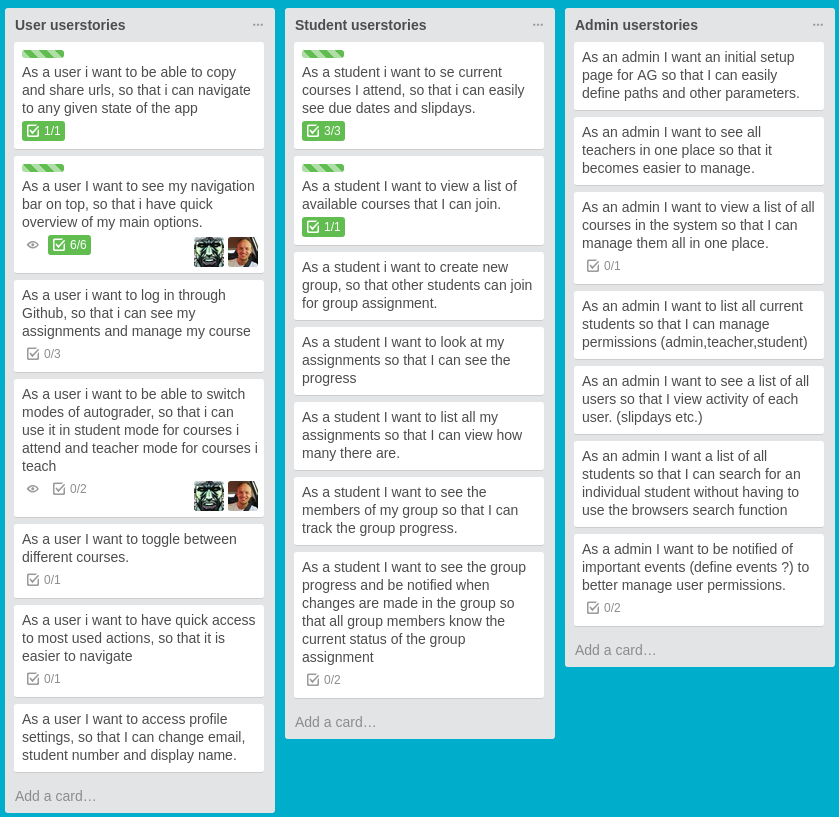
\includegraphics[width=0.8\textwidth]{./graphics/trello.png}
    \caption{Autograder's Trello page. Comprised of user stories, it was used as a TODO-list in the development process. Note: this is meant as an illustrative figure.}
    \label{fig:View of the trello page we used in the development process}
\end{figure}

\subsection{Wireframes}
The user stories are written down as cards. The user stories are then transformed into Wireframes. Wireframes are basic sketches or mockups of the design. The most basic forms doesn't include colors or advanced shapes. Simple boxes and rectangles are used to get a feel for how the page will look and function.
\\The wireframes are not to be confused with the design process. The wireframes are guides for user experience, not design. Having used the old Autograder system, we could use this previous experience to remake some of the layout. Examples of wireframes and the used in Autograder's development process will be presented later.

\subsection{Requirements collection and analysis}
Finding the requirements for Autograders new front-end is an important part of the development process. Our process of finding these requirements include talking to the client, Hein Meling at UiS. The requirements analysis is used to find expectations from the client, as well as the end users. Having used the Autograder system in a previous course at UiS, we were familiar with it's functions. 
Having discussed the user interface with other students, we already had some thoughts on how we could improve the front-end. Requirements for the new front-end was written down, mostly in the form of user stories from the beginning. Some of these requirements are not implemented in the Autograder prototype.

\subsubsection{User interface requirements}
\begin{itemize}
\item Users must be able to view the courses they can attend and request access to the courses.
\item Users must be able to select a course they attend and view progress of assignments and labs.
\item The progress, both for student and teachers, must be shown in an intuitive way.
\item Teachers must be able to approve and remove approval of assignments.
\item Both students and teachers must have a way of rebuilding the labs (button).
\item System maintainers and admins must be able to view all courses, students and teachers.
\end{itemize}

\subsubsection{Dummy data server requirements}
\begin{itemize}
\item A connection with the storage system must be set up.
\item A connection with the client must be set up for multiple connections at a time.
\item The server will handle multiple connections, and must be able to handle these in a concurrent way without overwriting data for other users.
\item Data must be transformed from the storage's format to a front-end compatible format.
\item The data must be in a format that makes the transition from dummy-server to real server as easy as possible.
\item Data must come in using predefined methods, to prevent anomalies both server- and storage-side. Unexpected connections to the server must be handled.
\item Autograder is not suppost to serve as an alternative view of GitHub repositories, and must work together with GitHub to view the source code of labs.
\end{itemize}

\subsubsection{Dummy data storage requirements}
\begin{itemize}
\item The database must be relational to the point where it can mimic real world Autograder users and relations.
\item Getting the data from the storage must be simple, with predefined ways of communicating and handling the data that comes in.
\end{itemize}

\subsubsection{Security requirements}
Security is not the scope of this thesis, nor the new Autograder front-end prototype. Future work must include authentifications for users.

\subsubsection{API requirements}
\begin{itemize}
\item 
\item The protocols used in the communication should be in a fixed format.
\end{itemize}
\subsubsection{Requirements for using the system}
No requirements should be necessary for students using the system. The system should be intuitive enough for any user to use it.

\section{The user interface}

Using the user stories and requirements introduced in earlier chapters, a new Autograder front-end has been designed. A lot of time was spend figuring out how the users tasks and workflows can be improved. Having discussed this with Hein Meling, it was decided that extra time would be used on the layout of the four pages presented below, to improve these parts compared to the original Autograder.

\begin{description}
\item [Left panel] Used for "local" navigation within the currently selected course. Mainly used to hide content that is not relevant at the current time (i.e settings page, score page).
\item [Middle panel] The most important content is placed in the middle. This is usually a table or list of students or roles.
\item [Right panel] This panel shows extended information about what is in the middle panel. Actions in the middle panel triggers updates to the right panel.
\item [Course toggler] Placed above all the other panels, in the middle, it is used to toggle between active courses. All users will see this on the relevant pages. Designed to make switching between courses easier, it also removes the need to redirect to change courses.
\end{description}

\subsection{The homepage}
The homepage lists all the current courses for the logged in user. The courses shown depend on the roles of the user. Courses the user can join are also listed here, to make the option of attending a new course easily accessible. Users can also request teaching permissions from the frontpage.

\begin{figure}[h!]
	 \centering
   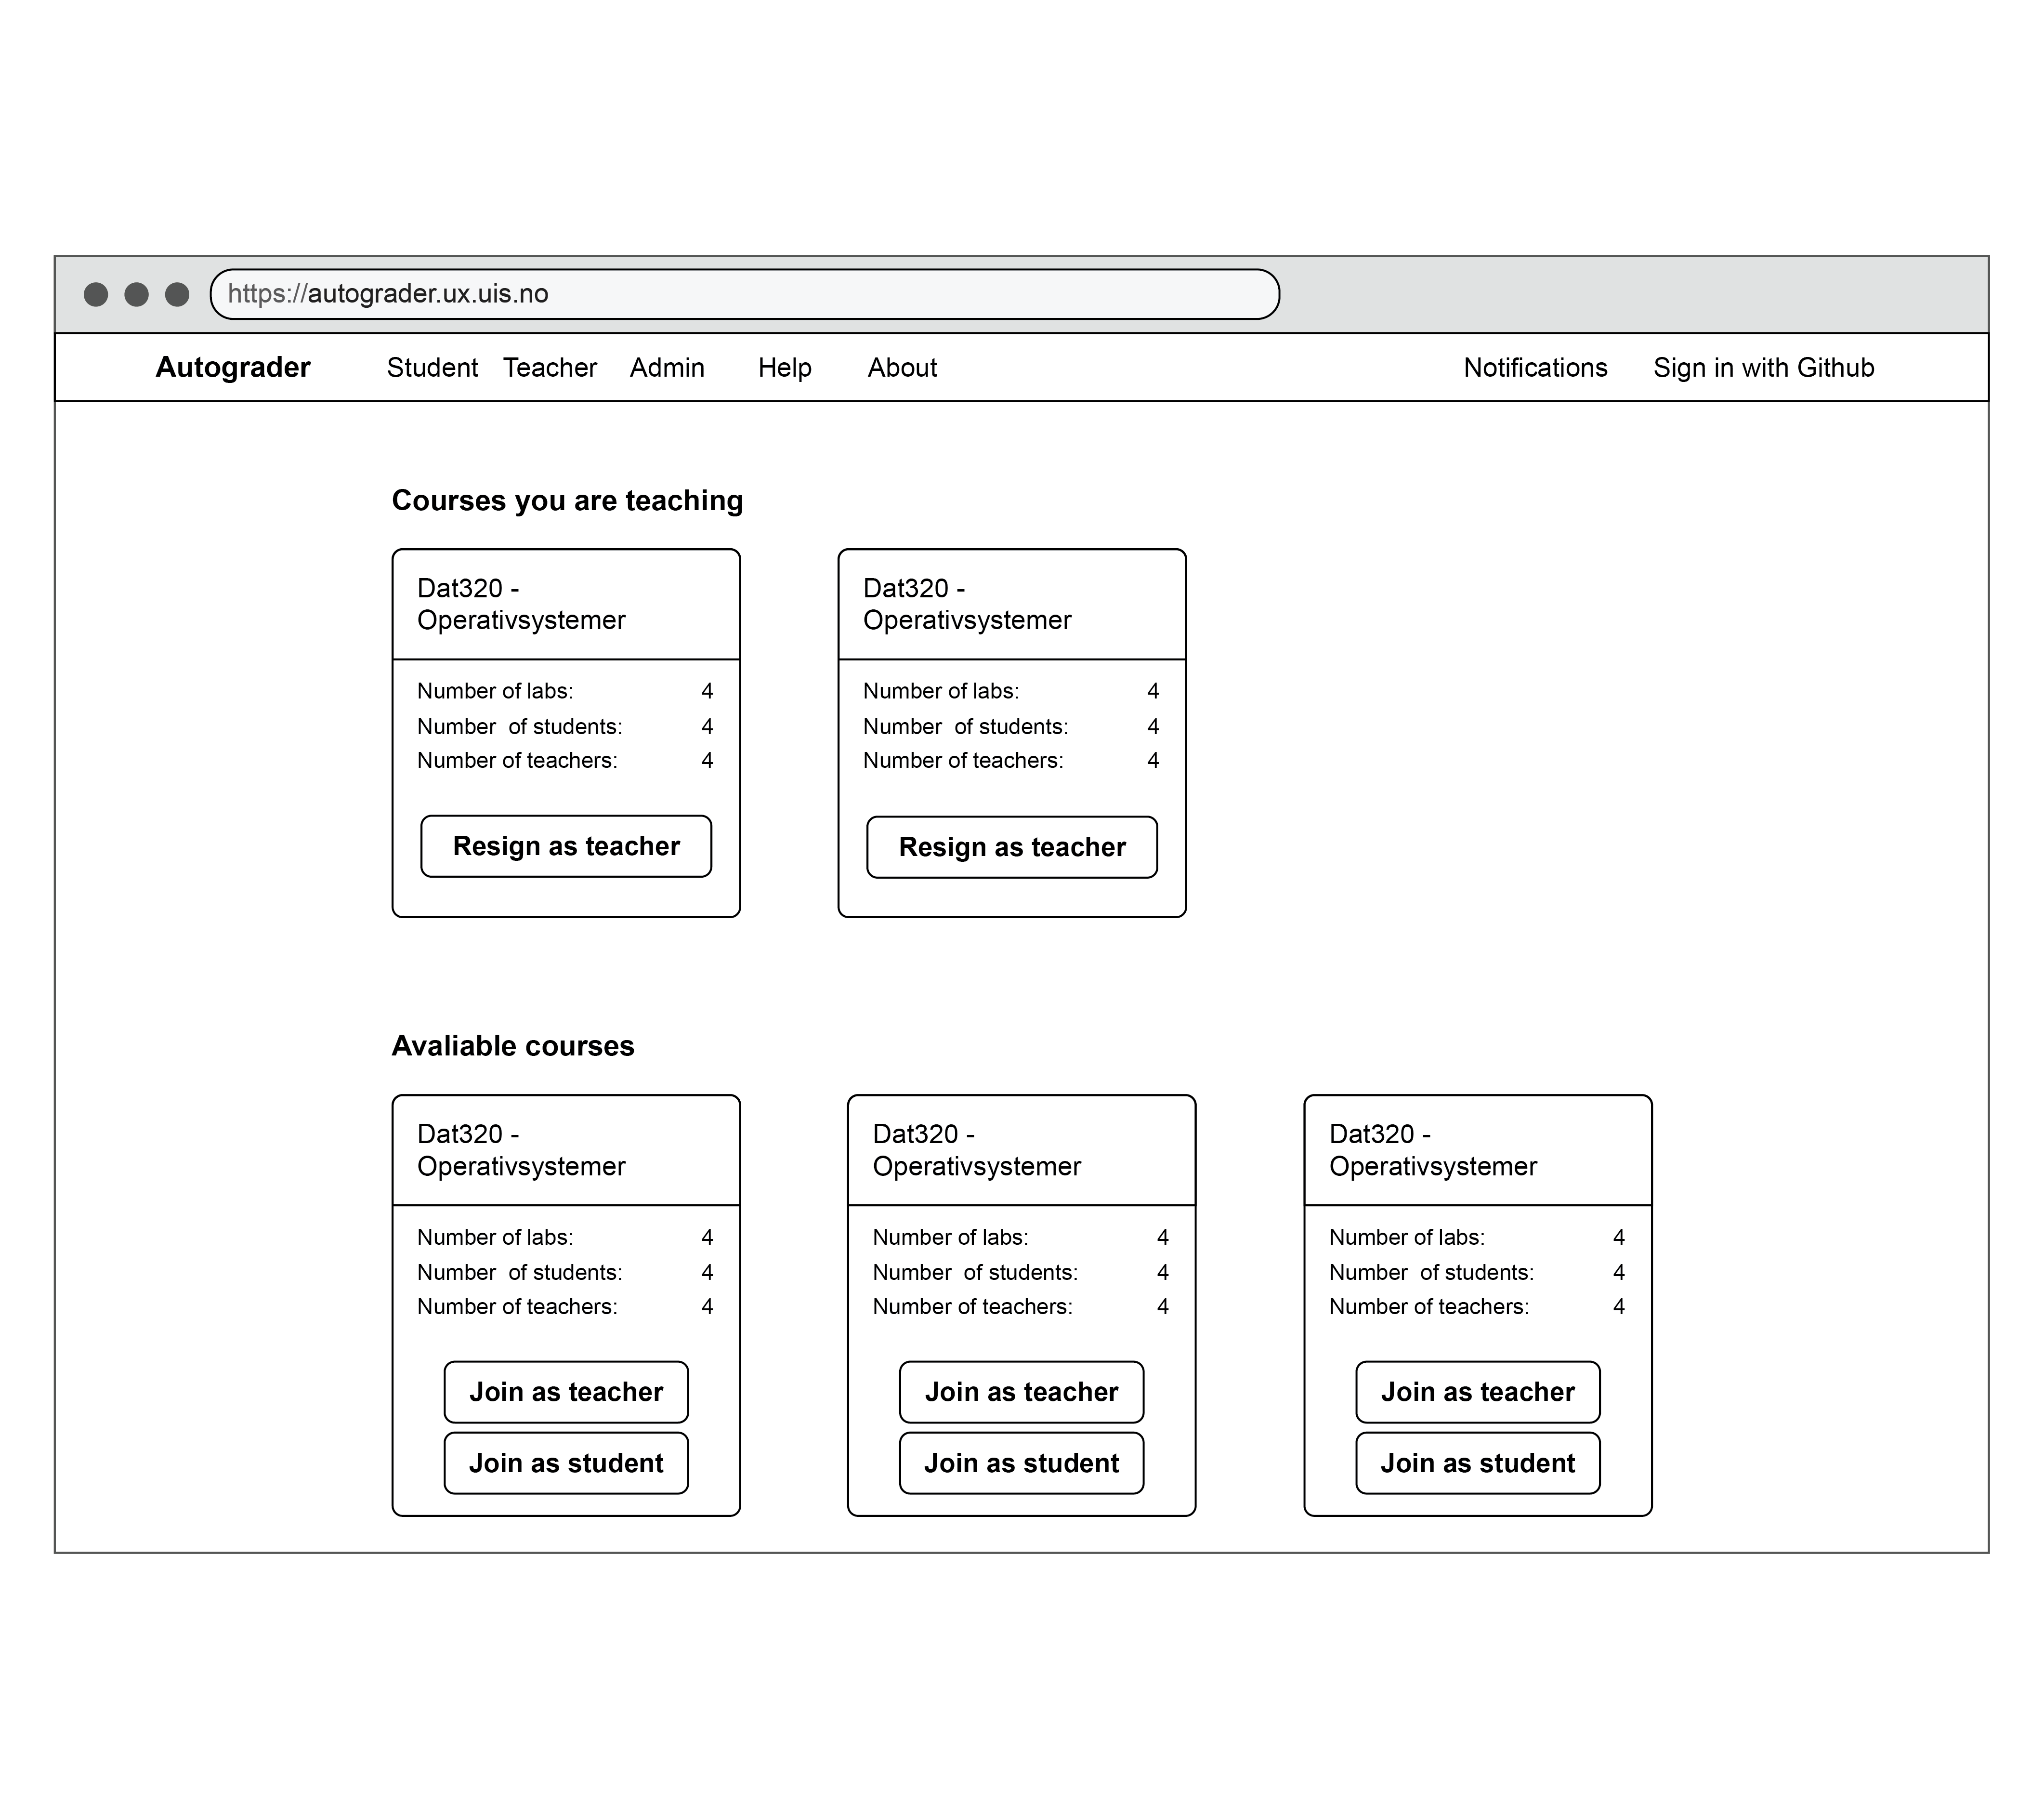
\includegraphics[width=1\textwidth]{homepage.png}
   \caption{The front page of the new Autograder}
   \label{fig:homepageAutograder}
\end{figure}

\ref{fig:homepageAutograder} shows the wireframe for the homepage of the new Autograder front-end. Each course has it's own card, with buttons for quick managment of user roles. Each card also shows some basic information from the course, such as the number of labs, students and teachers. Clicking on the card, will redirect the user to a course page where the selected course will be shown, including lab progress or a lab view (depending on the user role). As said, users can also view a list of all available courses as cards on the bottom of the page.

\subsection{The lab view}
The lab view has gone through several iterations, both in terms of design and layout. The original Autograder requires the teacher to visit each student's "page", where all the labs are listed for the currently selected student. The teacher grading the assignments has to go back end forth between the student page and the full list of students for every approval. Approving labs requires three redirects for every lab approved. Approving a class of 10 students requires 30 redirects, imagine a class of 50. The new Autograder front-end removes the need for page switching, by introducing the right side panel with lab view. Adding the right side "lab view panel" as seen in the wireframe, labs can be approved on the same page as the students are listed. A teacher can approve and view the lab results in the same window, for all students, removing the need to redirect the user.

\begin{figure}[h!]
   \centering
   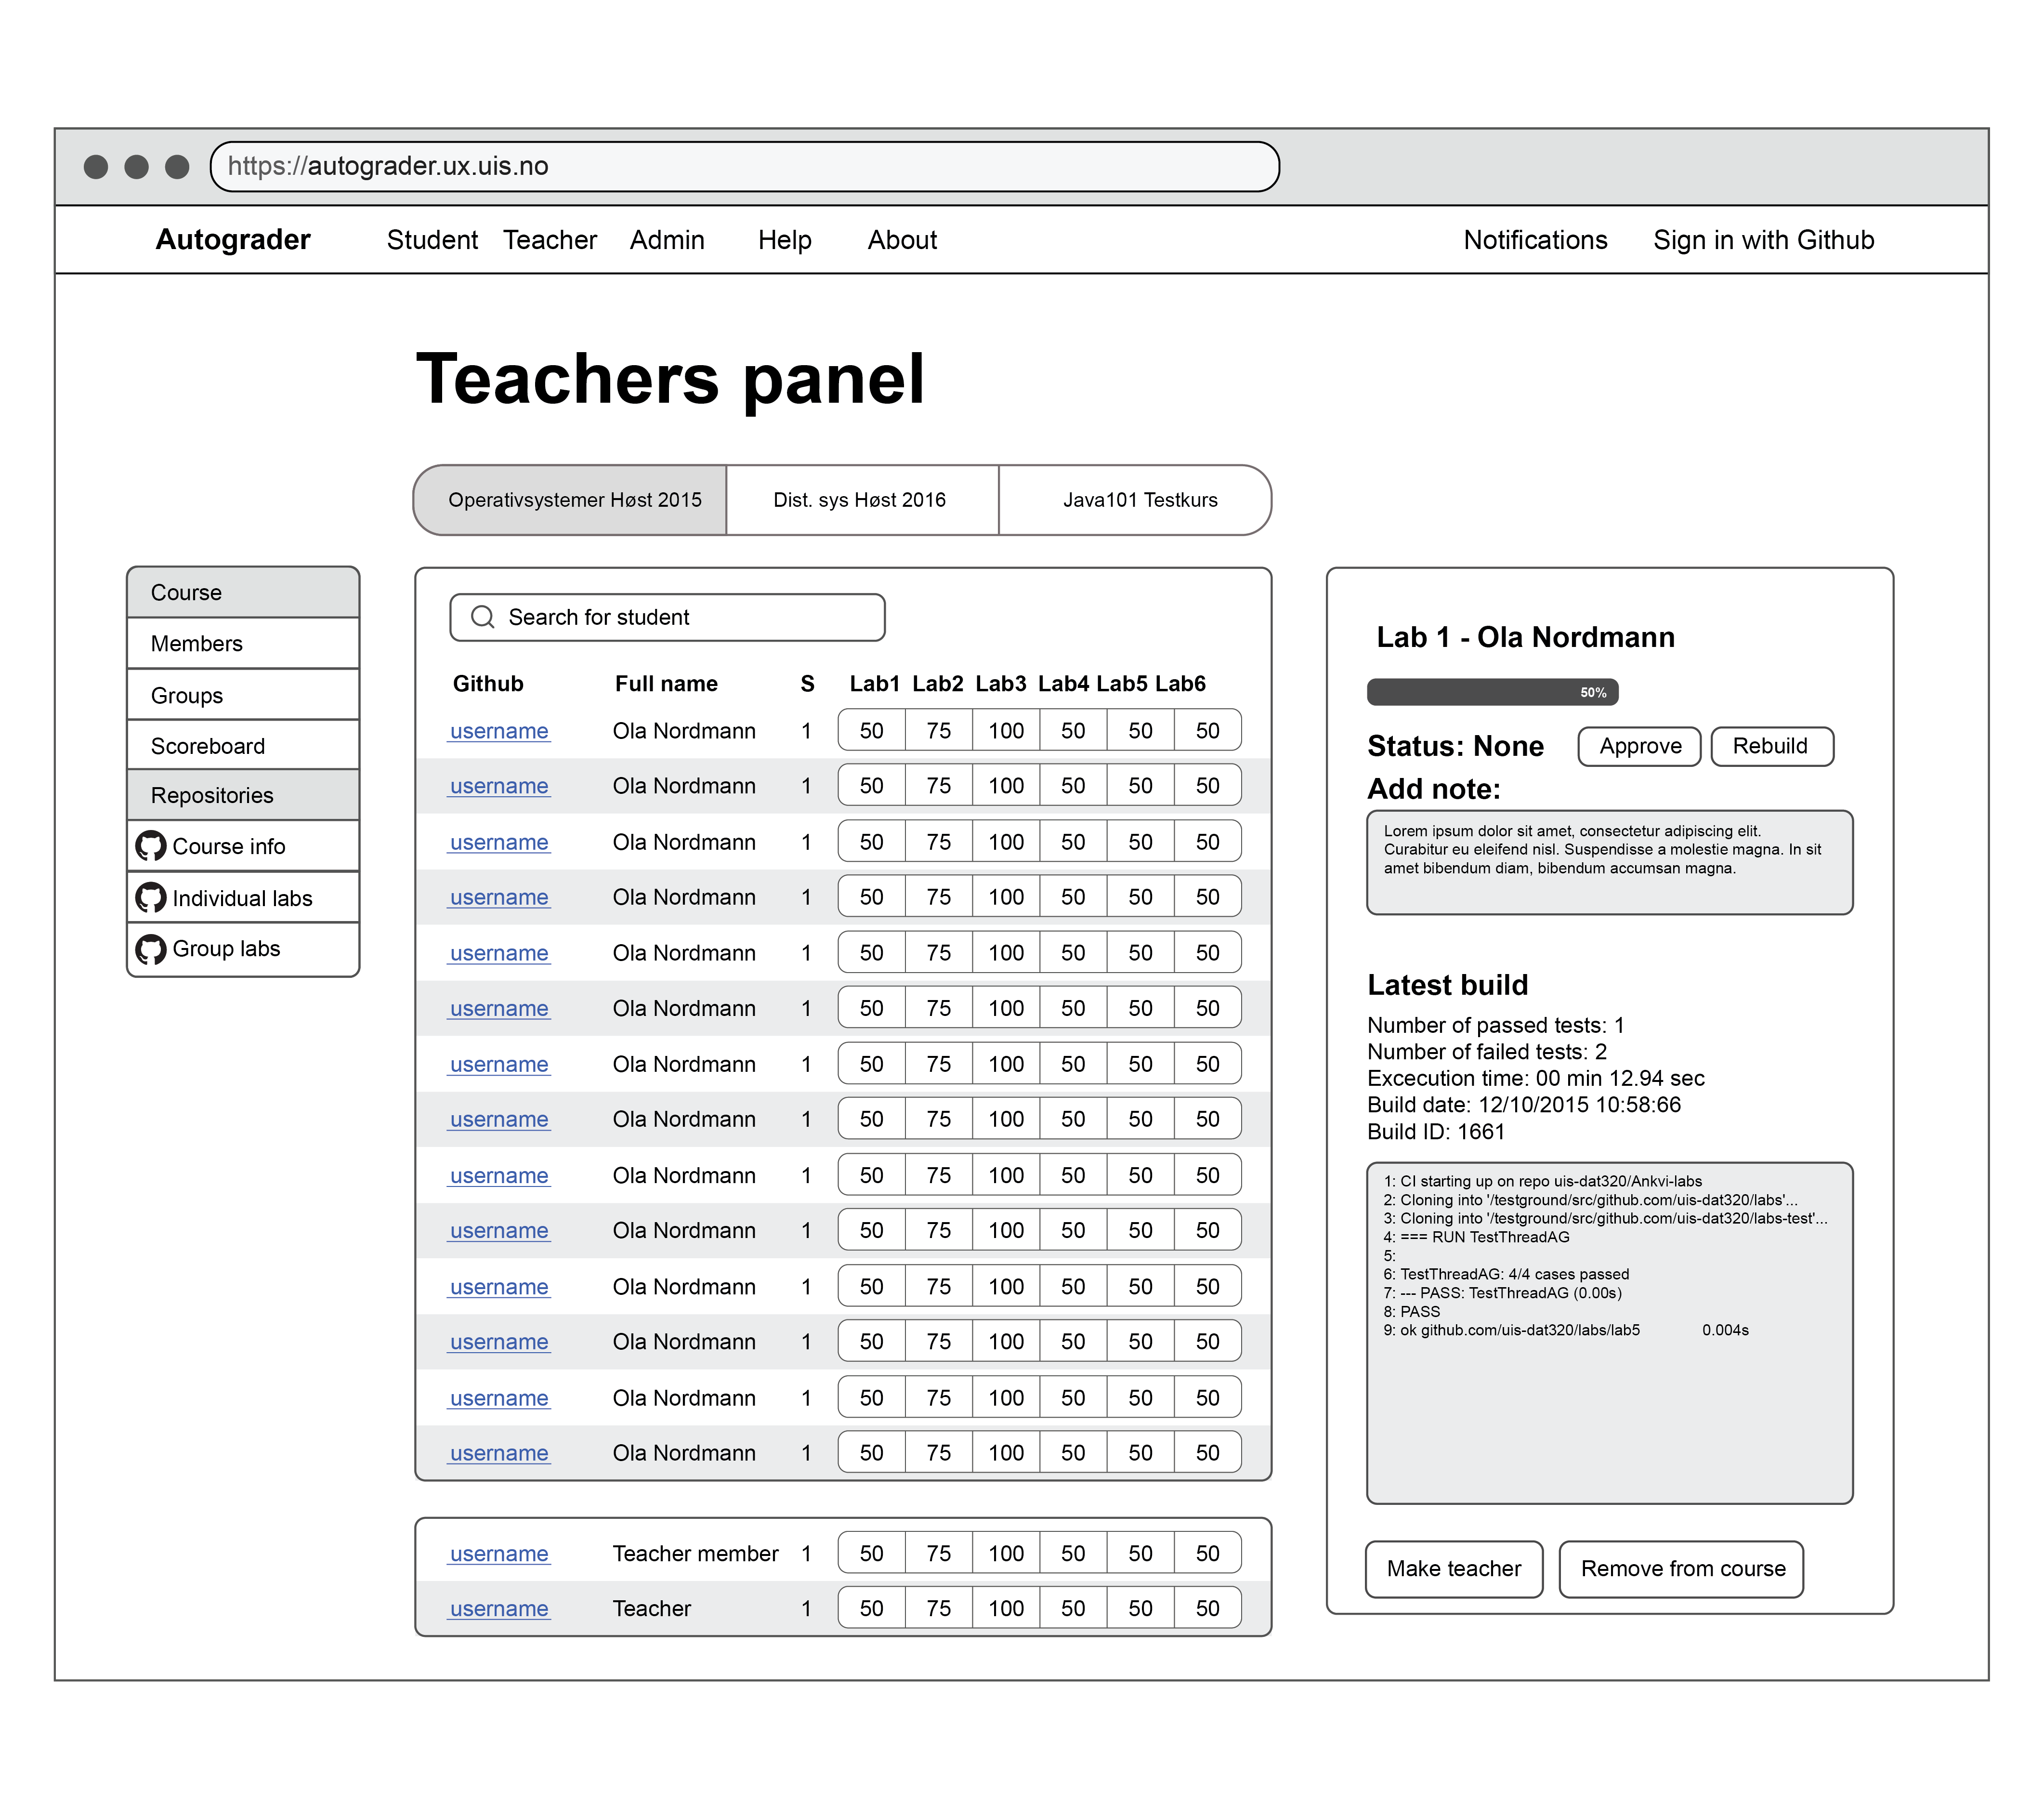
\includegraphics[width=1\textwidth]{labview.png}
   \caption{The view that teachers managing labs will have.}
   \label{fig:theLabView}
\end{figure}

The teacher panel, as seen in figure \ref{fig:theLabView}, is devided into four main parts. The left panel shows some navigation to other pages relevant for the teacher. The navigational bar over the middle panel, and under the header, is used to toggle between courses. This helps to remove unnecessary navigation between pages.

The middle panel shows all students in the currently selected course, as well as a search field. When a student is selected, the currently selected student will be updated, which will trigger an update in the right panel. The table form is used so that the number of labs can vary without effecting the layout of the page. When the number of labs exceed the amount of space assigned, the rest of the labs will be placed in a drop-down.

The right panel is designed to show the selected lab for a student, and triggers an update when the teacher clicks on another student. It is designed to show a summary of the currently selected lab, and implements functions to approve or rebuild the lab. A progress bar is also implemented, and will have visual guides to distinguish approved or failed labs. A build log is also implemented, and the results for the build process will be shown there. The teacher can also view an expanded view of the build log, which takes up the whole middle and right panel (not shown in the wireframe), to view a full log.

\subsection{Group manager}

Assignments that require groups can be created and managed in the group manager. The manager is designed to easily place students in groups. All the students in the course are listed in the middle panel. The right panel shows all groups and a button to create new groups. The teacher will select a group and add student in the selected group.

\begin{figure}[h!]
	 \centering
   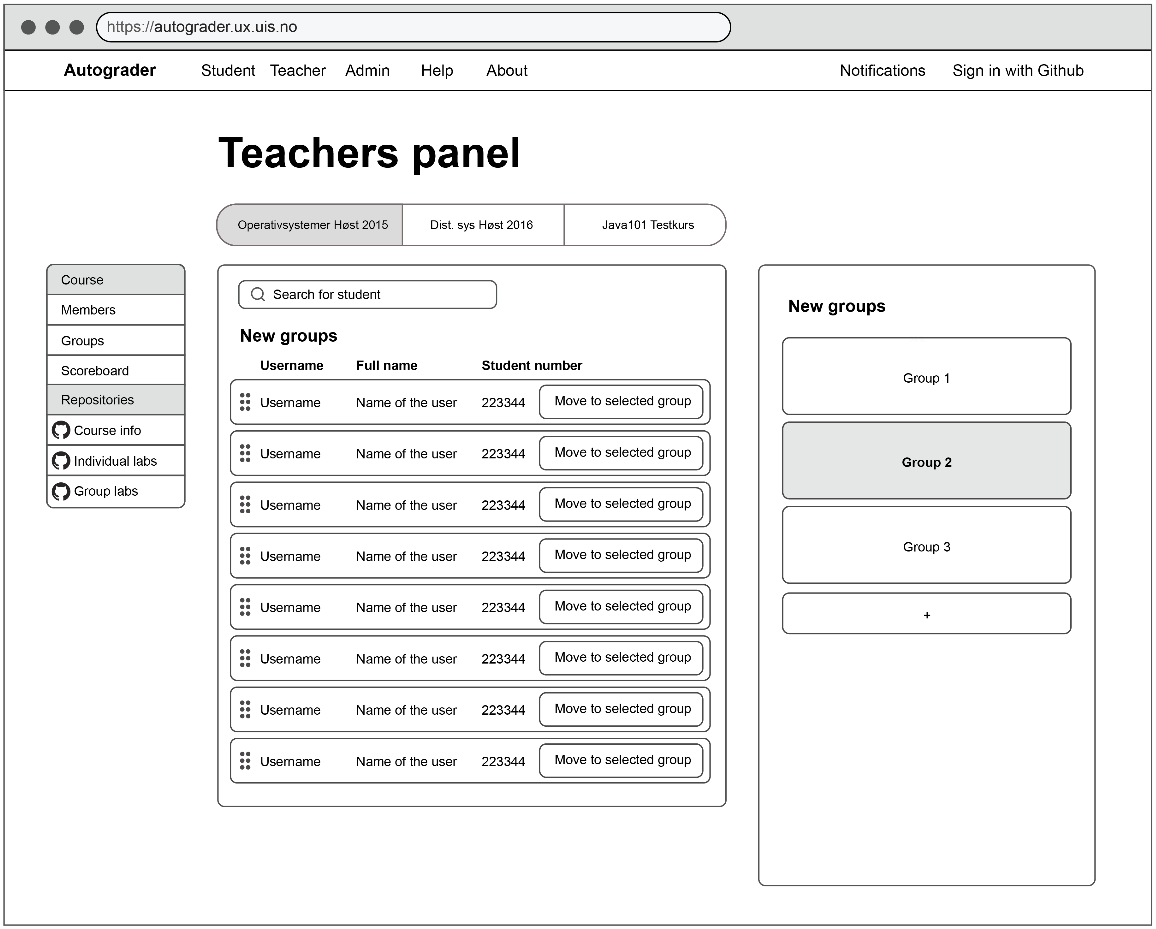
\includegraphics[width=1\textwidth]{groups.png}
   \caption{Group manager, seen as a wireframe.}
   \label{fig:groupManager}
\end{figure}


A requested feature from the client, Hein Meling, is that the teacher can use the group manager while the students are present in class. The teacher can go through the list of students, and place them in groups while the class i present, fast and simple. If the teacher chooses, it will also be possible to randomize groups. Another function of the group manager would be to implement a drag-and-drop, however, this is not implemented in the prototype. Figure \ref{fig:groupManager} shows the wireframe for the group manager.

\subsection{User manager}

\begin{figure}[h!]
	 \centering
   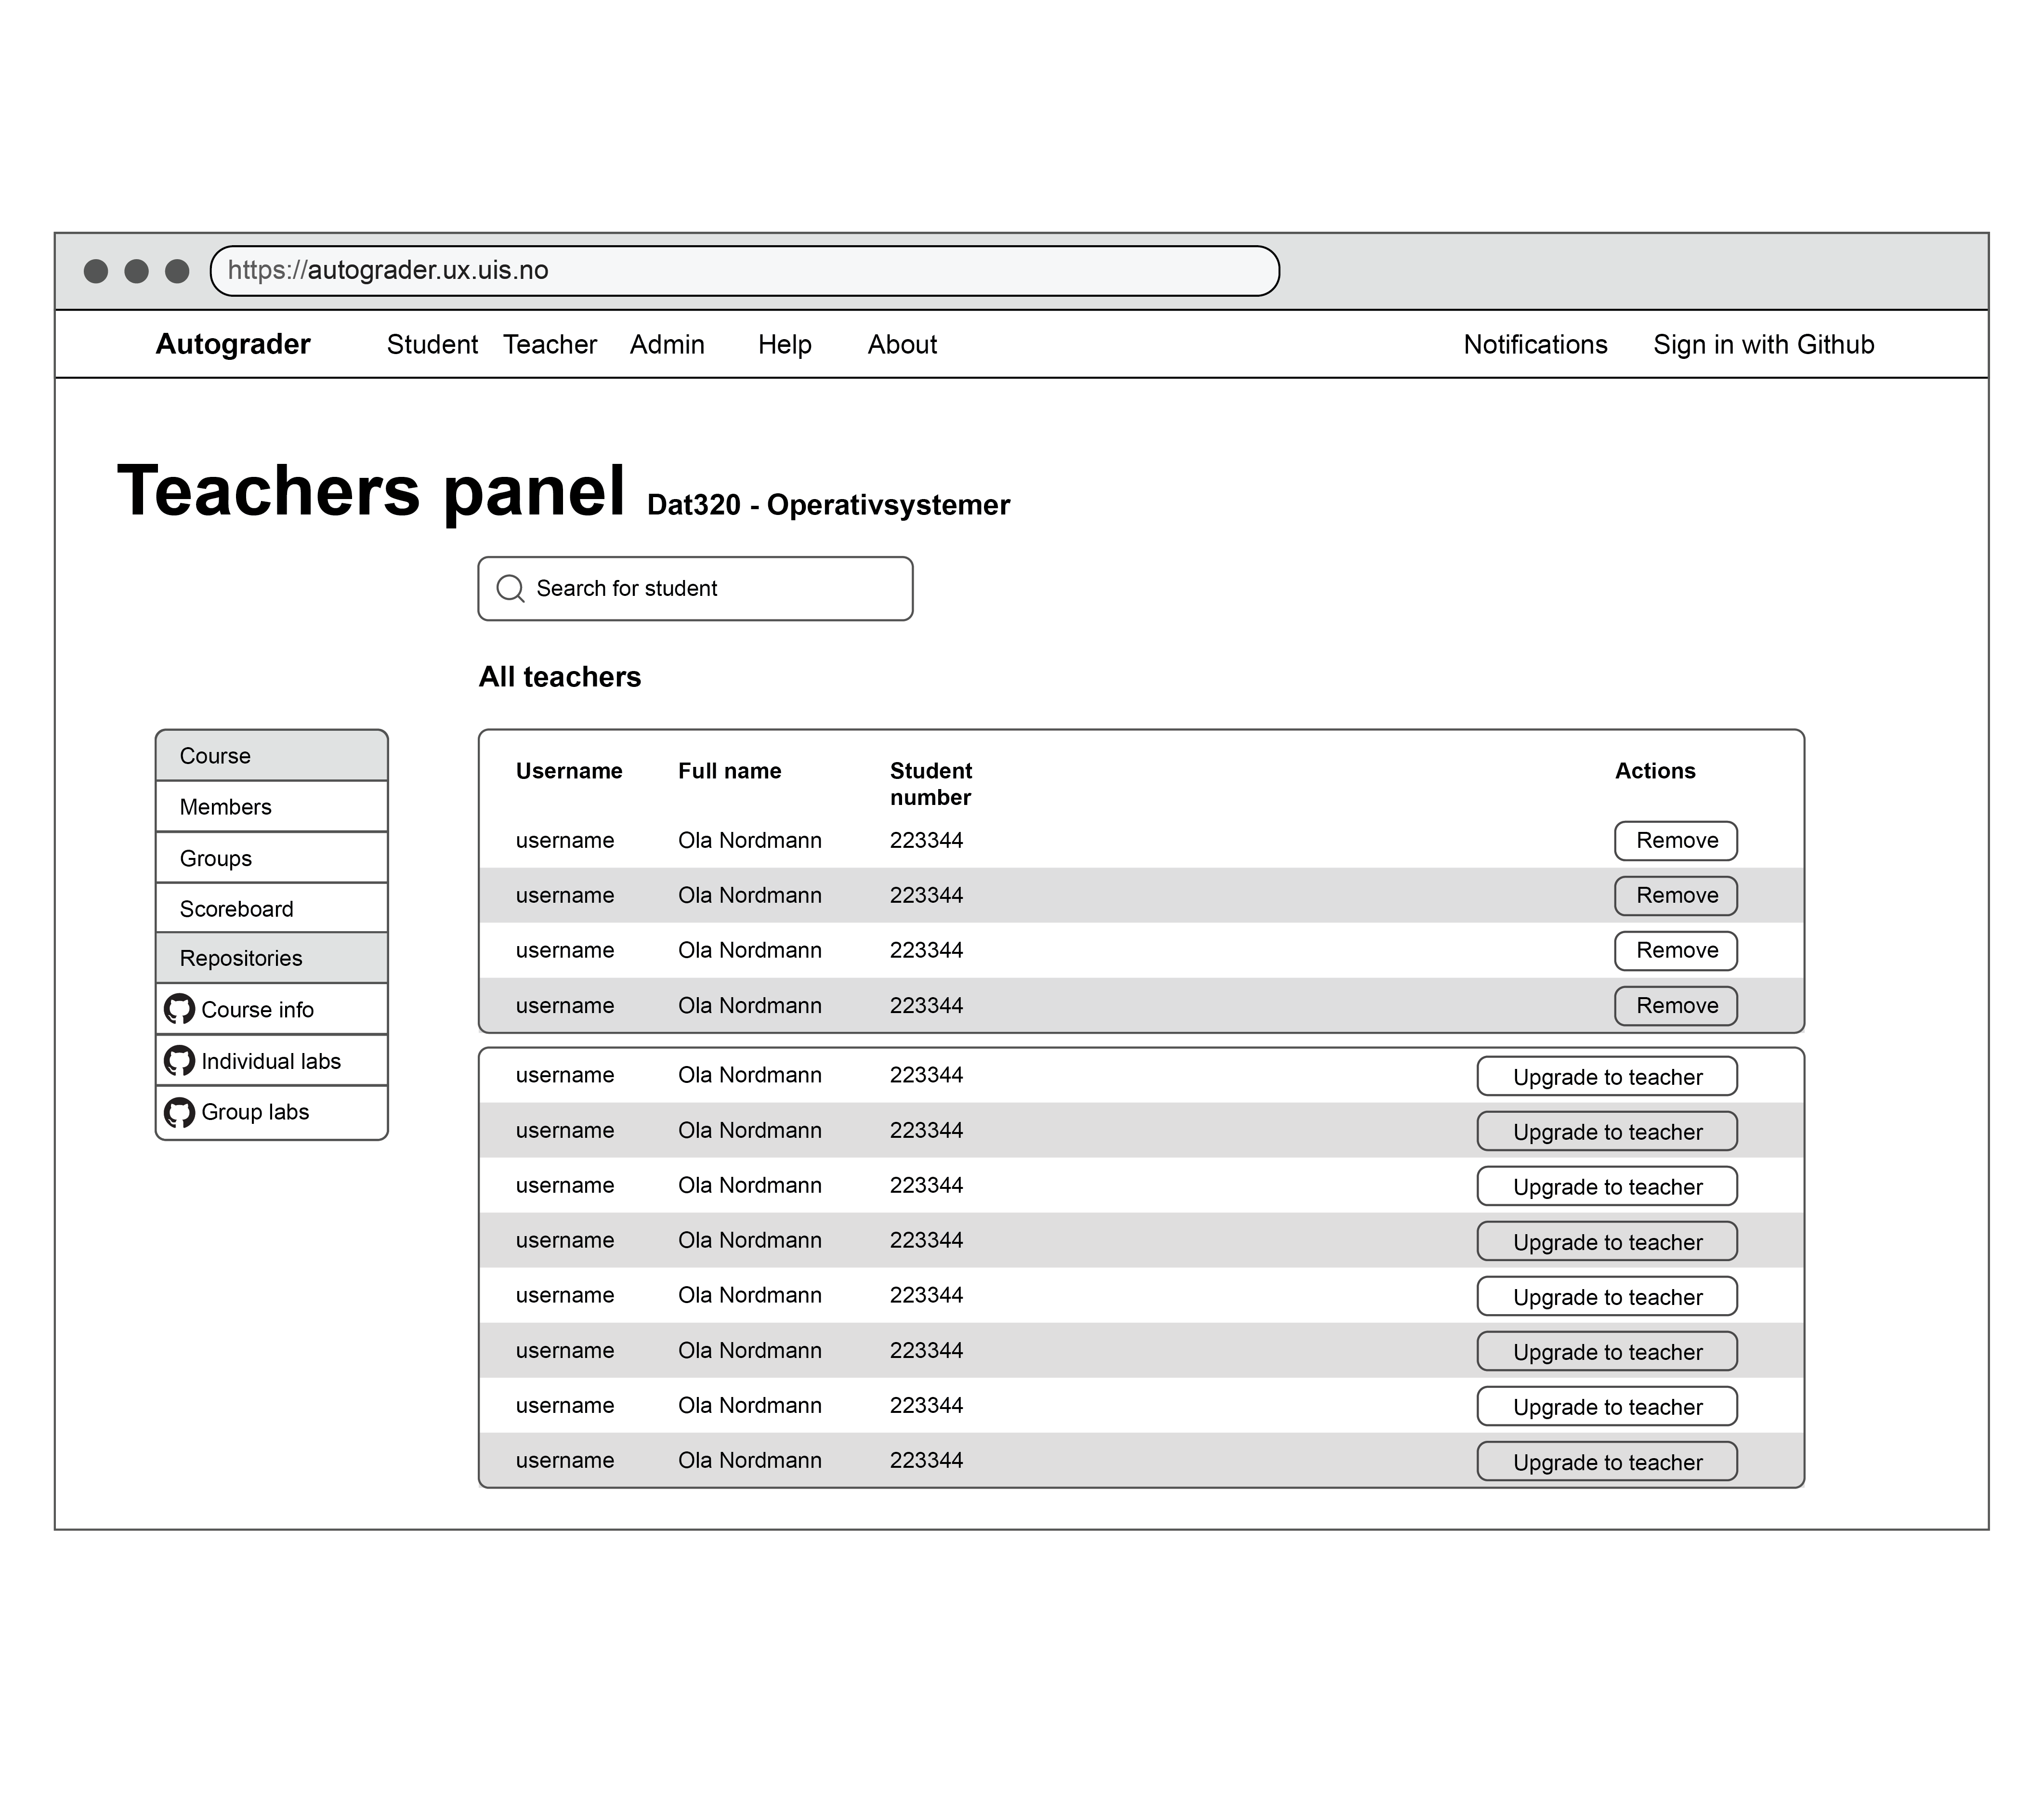
\includegraphics[width=1\textwidth]{roles.png}
   \caption{Page for managing roles in the system, specifically Admin, Teacher and Student}
   \label{fig:userManager}
\end{figure}

The figure \ref{fig:userManager} shows the layout of the user manager. The left panel is used to toggle between different roles in the system. The system maintainer will use this view to change permissions for the Autograder system and remove users. Toggling between roles is made easy with the left side panel (student,teacher). The middle panel will show all the users with the selected role, i.e students and teachers.










\section{Application architecture}
Choice of software architecture, software models for the front and back-end are crucial aspects of creating good application. This section will walk through the most important elements of the system, what it consists of and how different parts communicate with each other. Where did focus lay while developing it, what was done for testing purposes and for exploring future possibilities. Next the following subsections will dive a bit deeper into how the different parts worked individually, and briefly explain how the Autograder API works.

\subsection{Software architecture}
Autograder is an application for teachers and students. The new version is going to be running on a local university network and is going to be accessible from anywhere on the internet. Primary use for teachers is creating new courses in the system, that are associated with the courses at the university. Each course has a GitHub repository associated with it, and configured to the needs of that course. This means that Autograder's front-end and server must be designed to implement the GitHub integration.

\\Although the data is stored in the database, manipulation of that data is done on the client side first. It is then sent to the back-end for interpretation and trigger an  update in the database. Similarly it is also possible to update the client from the back-end, either directly or through the actions of another client. The user interface updates in real time, as an example, lets take a teacher that is assigning students to group assignments. The teacher is using an interactive interface to manipulate the users into selected groups, the student is simultaneously notified in real time when he gets assigned to a new group without the need to refresh the page. Teachers can be notified when a new student has enrolled in a course, or one of the students has exceeded his slip-days for an assignment. Real time updates are possible due to the connection protocol used in the application. When a client connects to the Autograder server, client application requests a protocol upgrade. From then on all data transfer is done through \emph{WebSocket protocol}\cite{websocket}. This enables the server to push its updates to all clients, without being explicitly asked for an update.
\\The reasoning behind real-time update system was that notifications and responsiveness of user interface was one of the primary reasons for developing the Autograder front-end. Although one could argue that other methods for updating the UI and notifications would be sufficient, like polling or long-polling - that is frequent client requests for update from the server. The WebSocket protocol has no obvious disadvantages to the presented solution, and at the same time opens possibilities for further upgrades of the system, like chat functionality, which could be utilized for questions related to assignments.

\subsection{The Autograder server and client}
The focus of this thesis is mostly front-end, although all the other parts should be mentioned and explained to give some context to the problem. Starting in with the back-end, the solution for server in the original Autograder is to have a virtual machine running that will host the Autograder application. For this purpose "Docker" \cite{docker} is used which lets the system admin run multiple applications in securely isolated containers. The docker engine is running on a host server with host OS. This solution lets the administrator run multiple applications on the same host server. The other crucial part of Autograder server-side is GitHub integration. This is done with the help of GitHub API \cite{githubAPI}, it can be used to link GitHub users with Autograder users and enable fetching the delivered code via GitHub to Autograder system. The API will also serves as authentication service for the users. Users of Autograder will log in with their GitHub accounts using GitHub's OAuth authentication \cite{githuboauth} and give access to their information to Autograder.

\begin{figure}[h]
  \scalebox{1}{% Graphic for TeX using PGF
% Title: /home/tomgli/workspace/github.com/bachopp/thesis/files/chapters/design/graphics/systemoverview.dia
% Creator: Dia v0.97.3
% CreationDate: Tue May 10 16:59:48 2016
% For: tomgli
% \usepackage{tikz}
% The following commands are not supported in PSTricks at present
% We define them conditionally, so when they are implemented,
% this pgf file will use them.
\ifx\du\undefined
  \newlength{\du}
\fi
\setlength{\du}{15\unitlength}
\begin{tikzpicture}
\pgftransformxscale{1.000000}
\pgftransformyscale{-1.000000}
\definecolor{dialinecolor}{rgb}{0.000000, 0.000000, 0.000000}
\pgfsetstrokecolor{dialinecolor}
\definecolor{dialinecolor}{rgb}{1.000000, 1.000000, 1.000000}
\pgfsetfillcolor{dialinecolor}
\definecolor{dialinecolor}{rgb}{1.000000, 1.000000, 1.000000}
\pgfsetfillcolor{dialinecolor}
\fill (27.326103\du,-25.722701\du)--(27.326103\du,-14.486061\du)--(33.132922\du,-14.486061\du)--(33.132922\du,-25.722701\du)--cycle;
\pgfsetlinewidth{0.100000\du}
\pgfsetdash{{\pgflinewidth}{0.200000\du}}{0cm}
\pgfsetdash{{\pgflinewidth}{0.200000\du}}{0cm}
\pgfsetmiterjoin
\definecolor{dialinecolor}{rgb}{0.525490, 0.525490, 0.525490}
\pgfsetstrokecolor{dialinecolor}
\draw (27.326103\du,-25.722701\du)--(27.326103\du,-14.486061\du)--(33.132922\du,-14.486061\du)--(33.132922\du,-25.722701\du)--cycle;
% setfont left to latex
\definecolor{dialinecolor}{rgb}{0.525490, 0.525490, 0.525490}
\pgfsetstrokecolor{dialinecolor}
\node at (30.229512\du,-19.909381\du){};
\definecolor{dialinecolor}{rgb}{1.000000, 1.000000, 1.000000}
\pgfsetfillcolor{dialinecolor}
\fill (26.419713\du,-25.405804\du)--(26.419713\du,-14.008996\du)--(32.226532\du,-14.008996\du)--(32.226532\du,-25.405804\du)--cycle;
\pgfsetlinewidth{0.100000\du}
\pgfsetdash{{\pgflinewidth}{0.200000\du}}{0cm}
\pgfsetdash{{\pgflinewidth}{0.200000\du}}{0cm}
\pgfsetmiterjoin
\definecolor{dialinecolor}{rgb}{0.525490, 0.525490, 0.525490}
\pgfsetstrokecolor{dialinecolor}
\draw (26.419713\du,-25.405804\du)--(26.419713\du,-14.008996\du)--(32.226532\du,-14.008996\du)--(32.226532\du,-25.405804\du)--cycle;
% setfont left to latex
\definecolor{dialinecolor}{rgb}{0.525490, 0.525490, 0.525490}
\pgfsetstrokecolor{dialinecolor}
\node at (29.323122\du,-19.512400\du){};
\pgfsetlinewidth{0.100000\du}
\pgfsetdash{{\pgflinewidth}{0.200000\du}}{0cm}
\pgfsetdash{{\pgflinewidth}{0.200000\du}}{0cm}
\pgfsetbuttcap
{
\definecolor{dialinecolor}{rgb}{0.525490, 0.525490, 0.525490}
\pgfsetfillcolor{dialinecolor}
% was here!!!
\definecolor{dialinecolor}{rgb}{0.525490, 0.525490, 0.525490}
\pgfsetstrokecolor{dialinecolor}
\draw (33.132922\du,-14.486061\du)--(29.906098\du,-10.809055\du);
}
\pgfsetlinewidth{0.100000\du}
\pgfsetdash{{\pgflinewidth}{0.200000\du}}{0cm}
\pgfsetdash{{\pgflinewidth}{0.200000\du}}{0cm}
\pgfsetbuttcap
{
\definecolor{dialinecolor}{rgb}{0.525490, 0.525490, 0.525490}
\pgfsetfillcolor{dialinecolor}
% was here!!!
\definecolor{dialinecolor}{rgb}{0.525490, 0.525490, 0.525490}
\pgfsetstrokecolor{dialinecolor}
\draw (32.226532\du,-14.008996\du)--(29.906098\du,-10.809055\du);
}
\pgfsetlinewidth{0.050000\du}
\pgfsetdash{}{0pt}
\pgfsetdash{}{0pt}
\pgfsetmiterjoin
\pgfsetbuttcap
{
\definecolor{dialinecolor}{rgb}{0.525490, 0.525490, 0.525490}
\pgfsetfillcolor{dialinecolor}
% was here!!!
\definecolor{dialinecolor}{rgb}{0.525490, 0.525490, 0.525490}
\pgfsetstrokecolor{dialinecolor}
\pgfpathmoveto{\pgfpoint{34.516603\du}{-15.824990\du}}
\pgfpathcurveto{\pgfpoint{34.097997\du}{-15.824990\du}}{\pgfpoint{33.088000\du}{-16.253649\du}}{\pgfpoint{32.669394\du}{-16.253649\du}}
\pgfusepath{stroke}
}
\pgfsetlinewidth{0.050000\du}
\pgfsetdash{}{0pt}
\pgfsetdash{}{0pt}
\pgfsetmiterjoin
\pgfsetbuttcap
{
\definecolor{dialinecolor}{rgb}{0.525490, 0.525490, 0.525490}
\pgfsetfillcolor{dialinecolor}
% was here!!!
\definecolor{dialinecolor}{rgb}{0.525490, 0.525490, 0.525490}
\pgfsetstrokecolor{dialinecolor}
\pgfpathmoveto{\pgfpoint{34.526280\du}{-15.821677\du}}
\pgfpathcurveto{\pgfpoint{34.107674\du}{-15.821677\du}}{\pgfpoint{32.146719\du}{-14.627397\du}}{\pgfpoint{31.728113\du}{-14.627397\du}}
\pgfusepath{stroke}
}
% setfont left to latex
\definecolor{dialinecolor}{rgb}{0.000000, 0.000000, 0.000000}
\pgfsetstrokecolor{dialinecolor}
\node[anchor=west] at (34.697393\du,-15.732157\du){docker instances};
\definecolor{dialinecolor}{rgb}{1.000000, 1.000000, 1.000000}
\pgfsetfillcolor{dialinecolor}
\fill (27.009049\du,-10.809055\du)--(27.009049\du,-7.364432\du)--(29.906098\du,-7.364432\du)--(29.906098\du,-10.809055\du)--cycle;
\pgfsetlinewidth{0.100000\du}
\pgfsetdash{{\pgflinewidth}{0.200000\du}}{0cm}
\pgfsetdash{{\pgflinewidth}{0.200000\du}}{0cm}
\pgfsetmiterjoin
\definecolor{dialinecolor}{rgb}{0.525490, 0.525490, 0.525490}
\pgfsetstrokecolor{dialinecolor}
\draw (27.009049\du,-10.809055\du)--(27.009049\du,-7.364432\du)--(29.906098\du,-7.364432\du)--(29.906098\du,-10.809055\du)--cycle;
% setfont left to latex
\definecolor{dialinecolor}{rgb}{0.525490, 0.525490, 0.525490}
\pgfsetstrokecolor{dialinecolor}
\node at (28.457574\du,-8.891744\du){};
% setfont left to latex
\definecolor{dialinecolor}{rgb}{0.525490, 0.525490, 0.525490}
\pgfsetstrokecolor{dialinecolor}
\node at (28.250862\du,-6.613056\du){Physical Server};
\definecolor{dialinecolor}{rgb}{1.000000, 1.000000, 1.000000}
\pgfsetfillcolor{dialinecolor}
\fill (25.473396\du,-25.096693\du)--(25.473396\du,-13.675219\du)--(31.280215\du,-13.675219\du)--(31.280215\du,-25.096693\du)--cycle;
\pgfsetlinewidth{0.100000\du}
\pgfsetdash{{\pgflinewidth}{0.200000\du}}{0cm}
\pgfsetdash{{\pgflinewidth}{0.200000\du}}{0cm}
\pgfsetmiterjoin
\definecolor{dialinecolor}{rgb}{0.525490, 0.525490, 0.525490}
\pgfsetstrokecolor{dialinecolor}
\draw (25.473396\du,-25.096693\du)--(25.473396\du,-13.675219\du)--(31.280215\du,-13.675219\du)--(31.280215\du,-25.096693\du)--cycle;
% setfont left to latex
\definecolor{dialinecolor}{rgb}{0.525490, 0.525490, 0.525490}
\pgfsetstrokecolor{dialinecolor}
\node at (28.376806\du,-19.190956\du){};
% setfont left to latex
\definecolor{dialinecolor}{rgb}{0.525490, 0.525490, 0.525490}
\pgfsetstrokecolor{dialinecolor}
\node[anchor=west] at (28.376806\du,-19.385956\du){};
\pgfsetlinewidth{0.100000\du}
\pgfsetdash{{\pgflinewidth}{0.200000\du}}{0cm}
\pgfsetdash{{\pgflinewidth}{0.200000\du}}{0cm}
\pgfsetbuttcap
{
\definecolor{dialinecolor}{rgb}{0.525490, 0.525490, 0.525490}
\pgfsetfillcolor{dialinecolor}
% was here!!!
\definecolor{dialinecolor}{rgb}{0.525490, 0.525490, 0.525490}
\pgfsetstrokecolor{dialinecolor}
\draw (31.280215\du,-13.675219\du)--(29.906098\du,-10.809055\du);
}
\pgfsetlinewidth{0.100000\du}
\pgfsetdash{{\pgflinewidth}{0.200000\du}}{0cm}
\pgfsetdash{{\pgflinewidth}{0.200000\du}}{0cm}
\pgfsetbuttcap
{
\definecolor{dialinecolor}{rgb}{0.525490, 0.525490, 0.525490}
\pgfsetfillcolor{dialinecolor}
% was here!!!
\definecolor{dialinecolor}{rgb}{0.525490, 0.525490, 0.525490}
\pgfsetstrokecolor{dialinecolor}
\draw (25.473396\du,-13.675219\du)--(27.009049\du,-10.809055\du);
}
\pgfsetlinewidth{0.100000\du}
\pgfsetdash{{\pgflinewidth}{0.200000\du}}{0cm}
\pgfsetdash{{\pgflinewidth}{0.200000\du}}{0cm}
\pgfsetbuttcap
{
\definecolor{dialinecolor}{rgb}{0.525490, 0.525490, 0.525490}
\pgfsetfillcolor{dialinecolor}
% was here!!!
\definecolor{dialinecolor}{rgb}{0.525490, 0.525490, 0.525490}
\pgfsetstrokecolor{dialinecolor}
\draw (26.241223\du,-12.242137\du)--(30.593157\du,-12.242137\du);
}
% setfont left to latex
\definecolor{dialinecolor}{rgb}{0.525490, 0.525490, 0.525490}
\pgfsetstrokecolor{dialinecolor}
\node at (28.507070\du,-11.296394\du){Host OS};
% setfont left to latex
\definecolor{dialinecolor}{rgb}{0.525490, 0.525490, 0.525490}
\pgfsetstrokecolor{dialinecolor}
\node at (28.320737\du,-13.135556\du){Docker Engine};
% setfont left to latex
\definecolor{dialinecolor}{rgb}{0.525490, 0.525490, 0.525490}
\pgfsetstrokecolor{dialinecolor}
\node[anchor=west] at (28.376806\du,-19.385956\du){};
% setfont left to latex
\definecolor{dialinecolor}{rgb}{0.525490, 0.525490, 0.525490}
\pgfsetstrokecolor{dialinecolor}
\node[anchor=west] at (28.692521\du,-11.345355\du){};
% setfont left to latex
\definecolor{dialinecolor}{rgb}{0.525490, 0.525490, 0.525490}
\pgfsetstrokecolor{dialinecolor}
\node at (28.262857\du,-14.170406\du){Autograder};
\pgfsetlinewidth{0.100000\du}
\pgfsetdash{{\pgflinewidth}{0.200000\du}}{0cm}
\pgfsetdash{{\pgflinewidth}{0.200000\du}}{0cm}
\pgfsetbuttcap
\pgfsetmiterjoin
\pgfsetlinewidth{0.100000\du}
\pgfsetbuttcap
\pgfsetmiterjoin
\pgfsetdash{{\pgflinewidth}{0.200000\du}}{0cm}
\definecolor{dialinecolor}{rgb}{1.000000, 1.000000, 1.000000}
\pgfsetfillcolor{dialinecolor}
\fill (27.006317\du,-10.189010\du)--(27.006317\du,-8.189010\du)--(29.916686\du,-8.189010\du)--(29.916686\du,-10.189010\du)--cycle;
\definecolor{dialinecolor}{rgb}{0.525490, 0.525490, 0.525490}
\pgfsetstrokecolor{dialinecolor}
\draw (27.006317\du,-10.189010\du)--(27.006317\du,-8.189010\du)--(29.916686\du,-8.189010\du)--(29.916686\du,-10.189010\du)--cycle;
\pgfsetbuttcap
\pgfsetmiterjoin
\pgfsetdash{{\pgflinewidth}{0.200000\du}}{0cm}
\definecolor{dialinecolor}{rgb}{0.525490, 0.525490, 0.525490}
\pgfsetstrokecolor{dialinecolor}
\draw (27.297354\du,-10.189010\du)--(27.297354\du,-8.189010\du);
\pgfsetbuttcap
\pgfsetmiterjoin
\pgfsetdash{{\pgflinewidth}{0.200000\du}}{0cm}
\definecolor{dialinecolor}{rgb}{0.525490, 0.525490, 0.525490}
\pgfsetstrokecolor{dialinecolor}
\draw (29.625649\du,-10.189010\du)--(29.625649\du,-8.189010\du);
% setfont left to latex
\definecolor{dialinecolor}{rgb}{0.525490, 0.525490, 0.525490}
\pgfsetstrokecolor{dialinecolor}
\node at (28.461502\du,-8.989010\du){};
\definecolor{dialinecolor}{rgb}{1.000000, 1.000000, 1.000000}
\pgfsetfillcolor{dialinecolor}
\fill (36.092879\du,-23.416305\du)--(36.092879\du,-21.314108\du)--(39.897856\du,-21.314108\du)--(39.897856\du,-23.416305\du)--cycle;
\pgfsetlinewidth{0.100000\du}
\pgfsetdash{{\pgflinewidth}{0.200000\du}}{0cm}
\pgfsetdash{{\pgflinewidth}{0.200000\du}}{0cm}
\pgfsetmiterjoin
\definecolor{dialinecolor}{rgb}{0.525490, 0.525490, 0.525490}
\pgfsetstrokecolor{dialinecolor}
\draw (36.092879\du,-23.416305\du)--(36.092879\du,-21.314108\du)--(39.897856\du,-21.314108\du)--(39.897856\du,-23.416305\du)--cycle;
% setfont left to latex
\definecolor{dialinecolor}{rgb}{0.525490, 0.525490, 0.525490}
\pgfsetstrokecolor{dialinecolor}
\node at (37.995367\du,-22.165206\du){GitHub};
\pgfsetlinewidth{0.100000\du}
\pgfsetdash{{1.000000\du}{1.000000\du}}{0\du}
\pgfsetdash{{1.000000\du}{1.000000\du}}{0\du}
\pgfsetbuttcap
{
\definecolor{dialinecolor}{rgb}{0.701961, 0.701961, 0.701961}
\pgfsetfillcolor{dialinecolor}
% was here!!!
\definecolor{dialinecolor}{rgb}{0.701961, 0.701961, 0.701961}
\pgfsetstrokecolor{dialinecolor}
\draw (30.789969\du,-22.890756\du)--(36.092879\du,-22.890756\du);
}
% setfont left to latex
\definecolor{dialinecolor}{rgb}{0.525490, 0.525490, 0.525490}
\pgfsetstrokecolor{dialinecolor}
\node[anchor=west] at (31.183820\du,-23.399697\du){GitHub API};
% setfont left to latex
\definecolor{dialinecolor}{rgb}{0.525490, 0.525490, 0.525490}
\pgfsetstrokecolor{dialinecolor}
\node at (34.610533\du,-22.310545\du){oauth};
\definecolor{dialinecolor}{rgb}{1.000000, 1.000000, 1.000000}
\pgfsetfillcolor{dialinecolor}
\fill (16.200243\du,-24.021230\du)--(16.200243\du,-21.175625\du)--(19.881608\du,-21.175625\du)--(19.881608\du,-24.021230\du)--cycle;
\pgfsetlinewidth{0.100000\du}
\pgfsetdash{}{0pt}
\pgfsetdash{}{0pt}
\pgfsetmiterjoin
\definecolor{dialinecolor}{rgb}{0.000000, 0.000000, 0.000000}
\pgfsetstrokecolor{dialinecolor}
\draw (16.200243\du,-24.021230\du)--(16.200243\du,-21.175625\du)--(19.881608\du,-21.175625\du)--(19.881608\du,-24.021230\du)--cycle;
% setfont left to latex
\definecolor{dialinecolor}{rgb}{0.000000, 0.000000, 0.000000}
\pgfsetstrokecolor{dialinecolor}
\node at (18.040926\du,-22.398427\du){Client};
\definecolor{dialinecolor}{rgb}{1.000000, 1.000000, 1.000000}
\pgfsetfillcolor{dialinecolor}
\fill (26.262677\du,-23.499667\du)--(26.262677\du,-19.954796\du)--(30.801821\du,-19.954796\du)--(30.801821\du,-23.499667\du)--cycle;
\pgfsetlinewidth{0.100000\du}
\pgfsetdash{}{0pt}
\pgfsetdash{}{0pt}
\pgfsetmiterjoin
\definecolor{dialinecolor}{rgb}{0.000000, 0.000000, 0.000000}
\pgfsetstrokecolor{dialinecolor}
\draw (26.262677\du,-23.499667\du)--(26.262677\du,-19.954796\du)--(30.801821\du,-19.954796\du)--(30.801821\du,-23.499667\du)--cycle;
% setfont left to latex
\definecolor{dialinecolor}{rgb}{0.000000, 0.000000, 0.000000}
\pgfsetstrokecolor{dialinecolor}
\node at (28.532249\du,-21.527232\du){Server};
\pgfsetlinewidth{0.100000\du}
\pgfsetdash{}{0pt}
\pgfsetdash{}{0pt}
\pgfsetbuttcap
{
\definecolor{dialinecolor}{rgb}{0.000000, 0.000000, 0.000000}
\pgfsetfillcolor{dialinecolor}
% was here!!!
\definecolor{dialinecolor}{rgb}{0.000000, 0.000000, 0.000000}
\pgfsetstrokecolor{dialinecolor}
\draw (19.881608\du,-22.598427\du)--(26.262677\du,-22.613449\du);
}
\pgfsetlinewidth{0.100000\du}
\pgfsetdash{}{0pt}
\pgfsetdash{}{0pt}
\pgfsetmiterjoin
\pgfsetbuttcap
{
\definecolor{dialinecolor}{rgb}{0.000000, 0.000000, 0.000000}
\pgfsetfillcolor{dialinecolor}
% was here!!!
{\pgfsetcornersarced{\pgfpoint{0.000000\du}{0.000000\du}}\definecolor{dialinecolor}{rgb}{0.000000, 0.000000, 0.000000}
\pgfsetstrokecolor{dialinecolor}
\draw (20.392143\du,-19.310304\du)--(21.533896\du,-19.312335\du)--(21.524315\du,-21.721982\du)--(26.262677\du,-21.727232\du);
}}
\pgfsetlinewidth{0.100000\du}
\pgfsetdash{}{0pt}
\pgfsetdash{}{0pt}
\pgfsetmiterjoin
\pgfsetbuttcap
{
\definecolor{dialinecolor}{rgb}{0.000000, 0.000000, 0.000000}
\pgfsetfillcolor{dialinecolor}
% was here!!!
{\pgfsetcornersarced{\pgfpoint{0.000000\du}{0.000000\du}}\definecolor{dialinecolor}{rgb}{0.000000, 0.000000, 0.000000}
\pgfsetstrokecolor{dialinecolor}
\draw (20.473663\du,-16.073804\du)--(22.382083\du,-16.073804\du)--(22.372836\du,-20.838105\du)--(26.262677\du,-20.841014\du);
}}
\definecolor{dialinecolor}{rgb}{1.000000, 1.000000, 1.000000}
\pgfsetfillcolor{dialinecolor}
\fill (25.735300\du,-23.269096\du)--(25.735300\du,-20.225449\du)--(26.835300\du,-20.225449\du)--(26.835300\du,-23.269096\du)--cycle;
\pgfsetlinewidth{0.100000\du}
\pgfsetdash{}{0pt}
\pgfsetdash{}{0pt}
\pgfsetmiterjoin
\definecolor{dialinecolor}{rgb}{0.000000, 0.000000, 0.000000}
\pgfsetstrokecolor{dialinecolor}
\draw (25.735300\du,-23.269096\du)--(25.735300\du,-20.225449\du)--(26.835300\du,-20.225449\du)--(26.835300\du,-23.269096\du)--cycle;
% setfont left to latex
\definecolor{dialinecolor}{rgb}{0.000000, 0.000000, 0.000000}
\pgfsetstrokecolor{dialinecolor}
\node at (26.285300\du,-21.552272\du){};
\pgfsetlinewidth{0.100000\du}
\pgfsetdash{}{0pt}
\pgfsetdash{}{0pt}
\pgfsetbuttcap
\pgfsetmiterjoin
\pgfsetlinewidth{0.100000\du}
\pgfsetbuttcap
\pgfsetmiterjoin
\pgfsetdash{}{0pt}
\definecolor{dialinecolor}{rgb}{1.000000, 1.000000, 1.000000}
\pgfsetfillcolor{dialinecolor}
\pgfpathmoveto{\pgfpoint{27.533916\du}{-17.013399\du}}
\pgfpathcurveto{\pgfpoint{27.933916\du}{-17.288399\du}}{\pgfpoint{28.133916\du}{-17.380065\du}}{\pgfpoint{28.533916\du}{-17.380065\du}}
\pgfpathcurveto{\pgfpoint{28.933916\du}{-17.380065\du}}{\pgfpoint{29.133916\du}{-17.288399\du}}{\pgfpoint{29.533916\du}{-17.013399\du}}
\pgfpathlineto{\pgfpoint{29.533916\du}{-15.546732\du}}
\pgfpathcurveto{\pgfpoint{29.133916\du}{-15.271732\du}}{\pgfpoint{28.933916\du}{-15.180065\du}}{\pgfpoint{28.533916\du}{-15.180065\du}}
\pgfpathcurveto{\pgfpoint{28.133916\du}{-15.180065\du}}{\pgfpoint{27.933916\du}{-15.271732\du}}{\pgfpoint{27.533916\du}{-15.546732\du}}
\pgfpathlineto{\pgfpoint{27.533916\du}{-17.013399\du}}
\pgfusepath{fill}
\definecolor{dialinecolor}{rgb}{0.000000, 0.000000, 0.000000}
\pgfsetstrokecolor{dialinecolor}
\pgfpathmoveto{\pgfpoint{27.533916\du}{-17.013399\du}}
\pgfpathcurveto{\pgfpoint{27.933916\du}{-17.288399\du}}{\pgfpoint{28.133916\du}{-17.380065\du}}{\pgfpoint{28.533916\du}{-17.380065\du}}
\pgfpathcurveto{\pgfpoint{28.933916\du}{-17.380065\du}}{\pgfpoint{29.133916\du}{-17.288399\du}}{\pgfpoint{29.533916\du}{-17.013399\du}}
\pgfpathlineto{\pgfpoint{29.533916\du}{-15.546732\du}}
\pgfpathcurveto{\pgfpoint{29.133916\du}{-15.271732\du}}{\pgfpoint{28.933916\du}{-15.180065\du}}{\pgfpoint{28.533916\du}{-15.180065\du}}
\pgfpathcurveto{\pgfpoint{28.133916\du}{-15.180065\du}}{\pgfpoint{27.933916\du}{-15.271732\du}}{\pgfpoint{27.533916\du}{-15.546732\du}}
\pgfpathlineto{\pgfpoint{27.533916\du}{-17.013399\du}}
\pgfusepath{stroke}
\pgfsetbuttcap
\pgfsetmiterjoin
\pgfsetdash{}{0pt}
\definecolor{dialinecolor}{rgb}{0.000000, 0.000000, 0.000000}
\pgfsetstrokecolor{dialinecolor}
\pgfpathmoveto{\pgfpoint{27.533916\du}{-17.013399\du}}
\pgfpathcurveto{\pgfpoint{27.933916\du}{-16.738399\du}}{\pgfpoint{28.133916\du}{-16.646732\du}}{\pgfpoint{28.533916\du}{-16.646732\du}}
\pgfpathcurveto{\pgfpoint{28.933916\du}{-16.646732\du}}{\pgfpoint{29.133916\du}{-16.738399\du}}{\pgfpoint{29.533916\du}{-17.013399\du}}
\pgfusepath{stroke}
% setfont left to latex
\definecolor{dialinecolor}{rgb}{0.000000, 0.000000, 0.000000}
\pgfsetstrokecolor{dialinecolor}
\node at (28.533916\du,-15.896732\du){DB};
\pgfsetlinewidth{0.100000\du}
\pgfsetdash{}{0pt}
\pgfsetdash{}{0pt}
\pgfsetbuttcap
{
\definecolor{dialinecolor}{rgb}{0.000000, 0.000000, 0.000000}
\pgfsetfillcolor{dialinecolor}
% was here!!!
\pgfsetarrowsstart{latex}
\pgfsetarrowsend{latex}
\definecolor{dialinecolor}{rgb}{0.000000, 0.000000, 0.000000}
\pgfsetstrokecolor{dialinecolor}
\draw (28.532249\du,-19.954796\du)--(28.533916\du,-17.380065\du);
}
% setfont left to latex
\definecolor{dialinecolor}{rgb}{0.000000, 0.000000, 0.000000}
\pgfsetstrokecolor{dialinecolor}
\node[anchor=west] at (21.845429\du,-23.167131\du){JSON};
% setfont left to latex
\definecolor{dialinecolor}{rgb}{0.000000, 0.000000, 0.000000}
\pgfsetstrokecolor{dialinecolor}
\node[anchor=west] at (28.730220\du,-18.390098\du){SQL};
\definecolor{dialinecolor}{rgb}{1.000000, 1.000000, 1.000000}
\pgfsetfillcolor{dialinecolor}
\fill (19.279304\du,-23.539801\du)--(19.279304\du,-21.639801\du)--(20.379304\du,-21.639801\du)--(20.379304\du,-23.539801\du)--cycle;
\pgfsetlinewidth{0.100000\du}
\pgfsetdash{}{0pt}
\pgfsetdash{}{0pt}
\pgfsetmiterjoin
\definecolor{dialinecolor}{rgb}{0.000000, 0.000000, 0.000000}
\pgfsetstrokecolor{dialinecolor}
\draw (19.279304\du,-23.539801\du)--(19.279304\du,-21.639801\du)--(20.379304\du,-21.639801\du)--(20.379304\du,-23.539801\du)--cycle;
% setfont left to latex
\definecolor{dialinecolor}{rgb}{0.000000, 0.000000, 0.000000}
\pgfsetstrokecolor{dialinecolor}
\node at (19.829304\du,-22.394801\du){};
\definecolor{dialinecolor}{rgb}{1.000000, 1.000000, 1.000000}
\pgfsetfillcolor{dialinecolor}
\fill (16.213082\du,-20.741732\du)--(16.213082\du,-17.896128\du)--(19.894447\du,-17.896128\du)--(19.894447\du,-20.741732\du)--cycle;
\pgfsetlinewidth{0.100000\du}
\pgfsetdash{}{0pt}
\pgfsetdash{}{0pt}
\pgfsetmiterjoin
\definecolor{dialinecolor}{rgb}{0.000000, 0.000000, 0.000000}
\pgfsetstrokecolor{dialinecolor}
\draw (16.213082\du,-20.741732\du)--(16.213082\du,-17.896128\du)--(19.894447\du,-17.896128\du)--(19.894447\du,-20.741732\du)--cycle;
% setfont left to latex
\definecolor{dialinecolor}{rgb}{0.000000, 0.000000, 0.000000}
\pgfsetstrokecolor{dialinecolor}
\node at (18.053765\du,-19.118930\du){Client};
\definecolor{dialinecolor}{rgb}{1.000000, 1.000000, 1.000000}
\pgfsetfillcolor{dialinecolor}
\fill (19.292143\du,-20.260304\du)--(19.292143\du,-18.360304\du)--(20.392143\du,-18.360304\du)--(20.392143\du,-20.260304\du)--cycle;
\pgfsetlinewidth{0.100000\du}
\pgfsetdash{}{0pt}
\pgfsetdash{}{0pt}
\pgfsetmiterjoin
\definecolor{dialinecolor}{rgb}{0.000000, 0.000000, 0.000000}
\pgfsetstrokecolor{dialinecolor}
\draw (19.292143\du,-20.260304\du)--(19.292143\du,-18.360304\du)--(20.392143\du,-18.360304\du)--(20.392143\du,-20.260304\du)--cycle;
% setfont left to latex
\definecolor{dialinecolor}{rgb}{0.000000, 0.000000, 0.000000}
\pgfsetstrokecolor{dialinecolor}
\node at (19.842143\du,-19.115304\du){};
\definecolor{dialinecolor}{rgb}{1.000000, 1.000000, 1.000000}
\pgfsetfillcolor{dialinecolor}
\fill (16.236465\du,-17.427168\du)--(16.236465\du,-14.581563\du)--(19.917830\du,-14.581563\du)--(19.917830\du,-17.427168\du)--cycle;
\pgfsetlinewidth{0.100000\du}
\pgfsetdash{}{0pt}
\pgfsetdash{}{0pt}
\pgfsetmiterjoin
\definecolor{dialinecolor}{rgb}{0.000000, 0.000000, 0.000000}
\pgfsetstrokecolor{dialinecolor}
\draw (16.236465\du,-17.427168\du)--(16.236465\du,-14.581563\du)--(19.917830\du,-14.581563\du)--(19.917830\du,-17.427168\du)--cycle;
% setfont left to latex
\definecolor{dialinecolor}{rgb}{0.000000, 0.000000, 0.000000}
\pgfsetstrokecolor{dialinecolor}
\node at (18.077148\du,-15.804365\du){Client};
\definecolor{dialinecolor}{rgb}{1.000000, 1.000000, 1.000000}
\pgfsetfillcolor{dialinecolor}
\fill (19.315526\du,-16.945739\du)--(19.315526\du,-15.045739\du)--(20.415526\du,-15.045739\du)--(20.415526\du,-16.945739\du)--cycle;
\pgfsetlinewidth{0.100000\du}
\pgfsetdash{}{0pt}
\pgfsetdash{}{0pt}
\pgfsetmiterjoin
\definecolor{dialinecolor}{rgb}{0.000000, 0.000000, 0.000000}
\pgfsetstrokecolor{dialinecolor}
\draw (19.315526\du,-16.945739\du)--(19.315526\du,-15.045739\du)--(20.415526\du,-15.045739\du)--(20.415526\du,-16.945739\du)--cycle;
% setfont left to latex
\definecolor{dialinecolor}{rgb}{0.000000, 0.000000, 0.000000}
\pgfsetstrokecolor{dialinecolor}
\node at (19.865526\du,-15.800739\du){};
\pgfsetlinewidth{0.050000\du}
\pgfsetdash{}{0pt}
\pgfsetdash{}{0pt}
\pgfsetmiterjoin
\pgfsetbuttcap
{
\definecolor{dialinecolor}{rgb}{0.000000, 0.000000, 0.000000}
\pgfsetfillcolor{dialinecolor}
% was here!!!
\definecolor{dialinecolor}{rgb}{0.000000, 0.000000, 0.000000}
\pgfsetstrokecolor{dialinecolor}
\pgfpathmoveto{\pgfpoint{26.226836\du}{-22.786437\du}}
\pgfpathcurveto{\pgfpoint{25.808230\du}{-22.786437\du}}{\pgfpoint{25.384581\du}{-27.119216\du}}{\pgfpoint{24.965975\du}{-27.119216\du}}
\pgfusepath{stroke}
}
% setfont left to latex
\definecolor{dialinecolor}{rgb}{0.000000, 0.000000, 0.000000}
\pgfsetstrokecolor{dialinecolor}
\node[anchor=west] at (22.535951\du,-27.210915\du){gorilla/websocket};
% setfont left to latex
\definecolor{dialinecolor}{rgb}{0.000000, 0.000000, 0.000000}
\pgfsetstrokecolor{dialinecolor}
\node at (19.833576\du,-23.001849\du){ws};
% setfont left to latex
\definecolor{dialinecolor}{rgb}{0.000000, 0.000000, 0.000000}
\pgfsetstrokecolor{dialinecolor}
\node at (19.862753\du,-19.685082\du){ws};
% setfont left to latex
\definecolor{dialinecolor}{rgb}{0.000000, 0.000000, 0.000000}
\pgfsetstrokecolor{dialinecolor}
\node at (19.875721\du,-16.384763\du){ws};
% setfont left to latex
\definecolor{dialinecolor}{rgb}{0.000000, 0.000000, 0.000000}
\pgfsetstrokecolor{dialinecolor}
\node[anchor=west] at (15.442558\du,-24.575303\du){*ws = WebSocket};
\end{tikzpicture}
}
  \caption{Overview of the whole system, not implemented modules are grayed out.}
  \label{fig:systemoverview}
\end{figure}

The diagram shown in figure \ref{fig:systemoverview} represents the model of the whole Autograder system together with server solution, database, and GitHub integration. When the user goes to the Autograder page, it will use the integrated GitHub authentication to login and access the page. When the Authentication is confirmed, server can communicate with the remote repositories, fetch the data and run the tests prepared by the teacher, examine students assignments. GitHub is used solely for storing the students code. Data is only being obtained from the service new changes are not pushed to GitHub. When the server figures out what data to get and associates it with the correct user data from the Autograder database, and the test results return, it can update the front-end client.
\\Communication with the client happens through WebSocket. To implement it, a library called gorilla/websocket \cite{gorilla} is used. As explained earlier, the server implemented in this thesis is only used for testing out the client communication and transporting dummy data. This solution worked fine but other libraries and implementations should be considered in the future work. For database solution, we communicate with a MySQL server that runs locally, it is a separate process from the main Autograder server. The communication between server and the database is done with the help of Go libraries using SQL. Requests from client-side are first sent through WebSocket in JSON format to the server, then a function call to the database is invoked, next the database returns with no errors, and the correct response is send back to the client through the server.  

\subsection{The client}
Web client for the Autograder is written in JavaScript, with the help of React library. Together with Flux architecture, React gives a very good framework for building application-specific software with responsive interface. The web client utilizes a WebSocket protocol to exchange data with the server. When the client requests some information, an API is used to construct the message, then it gets wrapped in JSON format and send through established WebSocket connection.
\begin{figure}[h]
  \scalebox{1}{% Graphic for TeX using PGF
% Title: /home/tomgli/workspace/github.com/bachopp/thesis/files/chapters/design/graphics/clientoverview.dia
% Creator: Dia v0.97.3
% CreationDate: Thu May 12 14:50:22 2016
% For: tomgli
% \usepackage{tikz}
% The following commands are not supported in PSTricks at present
% We define them conditionally, so when they are implemented,
% this pgf file will use them.
\ifx\du\undefined
  \newlength{\du}
\fi
\setlength{\du}{15\unitlength}
\begin{tikzpicture}
\pgftransformxscale{1.000000}
\pgftransformyscale{-1.000000}
\definecolor{dialinecolor}{rgb}{0.000000, 0.000000, 0.000000}
\pgfsetstrokecolor{dialinecolor}
\definecolor{dialinecolor}{rgb}{1.000000, 1.000000, 1.000000}
\pgfsetfillcolor{dialinecolor}
% setfont left to latex
\definecolor{dialinecolor}{rgb}{0.000000, 0.000000, 0.000000}
\pgfsetstrokecolor{dialinecolor}
\node at (37.361400\du,-16.322550\du){WS};
\pgfsetlinewidth{0.100000\du}
\pgfsetdash{}{0pt}
\pgfsetdash{}{0pt}
\pgfsetmiterjoin
\pgfsetbuttcap
{
\definecolor{dialinecolor}{rgb}{0.000000, 0.000000, 0.000000}
\pgfsetfillcolor{dialinecolor}
% was here!!!
{\pgfsetcornersarced{\pgfpoint{0.000000\du}{0.000000\du}}\definecolor{dialinecolor}{rgb}{0.000000, 0.000000, 0.000000}
\pgfsetstrokecolor{dialinecolor}
\draw (36.616438\du,-18.569878\du)--(38.251100\du,-17.133800\du)--(38.251800\du,-16.155300\du)--(36.616438\du,-14.507751\du);
}}
\pgfsetlinewidth{0.100000\du}
\pgfsetdash{}{0pt}
\pgfsetdash{}{0pt}
\pgfsetbuttcap
{
\definecolor{dialinecolor}{rgb}{0.000000, 0.000000, 0.000000}
\pgfsetfillcolor{dialinecolor}
% was here!!!
\pgfsetarrowsend{latex}
\definecolor{dialinecolor}{rgb}{0.000000, 0.000000, 0.000000}
\pgfsetstrokecolor{dialinecolor}
\draw (38.266600\du,-17.117900\du)--(40.504300\du,-17.117200\du);
}
% setfont left to latex
\definecolor{dialinecolor}{rgb}{0.000000, 0.000000, 0.000000}
\pgfsetstrokecolor{dialinecolor}
\node at (41.484800\du,-16.452150\du){JSON};
\pgfsetlinewidth{0.100000\du}
\pgfsetdash{}{0pt}
\pgfsetdash{}{0pt}
\pgfsetbuttcap
{
\definecolor{dialinecolor}{rgb}{0.000000, 0.000000, 0.000000}
\pgfsetfillcolor{dialinecolor}
% was here!!!
\pgfsetarrowsstart{latex}
\definecolor{dialinecolor}{rgb}{0.000000, 0.000000, 0.000000}
\pgfsetstrokecolor{dialinecolor}
\draw (38.258400\du,-16.158400\du)--(40.496000\du,-16.157700\du);
}
\definecolor{dialinecolor}{rgb}{1.000000, 1.000000, 1.000000}
\pgfsetfillcolor{dialinecolor}
\fill (29.727479\du,-19.012100\du)--(29.727479\du,-14.092004\du)--(35.790613\du,-14.092004\du)--(35.790613\du,-19.012100\du)--cycle;
\pgfsetlinewidth{0.100000\du}
\pgfsetdash{}{0pt}
\pgfsetdash{}{0pt}
\pgfsetmiterjoin
\definecolor{dialinecolor}{rgb}{0.000000, 0.000000, 0.000000}
\pgfsetstrokecolor{dialinecolor}
\draw (29.727479\du,-19.012100\du)--(29.727479\du,-14.092004\du)--(35.790613\du,-14.092004\du)--(35.790613\du,-19.012100\du)--cycle;
% setfont left to latex
\definecolor{dialinecolor}{rgb}{0.000000, 0.000000, 0.000000}
\pgfsetstrokecolor{dialinecolor}
\node at (32.759046\du,-16.357052\du){};
% setfont left to latex
\definecolor{dialinecolor}{rgb}{0.000000, 0.000000, 0.000000}
\pgfsetstrokecolor{dialinecolor}
\node[anchor=west] at (31.692932\du,-16.294700\du){Client};
\definecolor{dialinecolor}{rgb}{1.000000, 1.000000, 1.000000}
\pgfsetfillcolor{dialinecolor}
\fill (34.441600\du,-18.569878\du)--(34.441600\du,-14.507751\du)--(36.616438\du,-14.507751\du)--(36.616438\du,-18.569878\du)--cycle;
\pgfsetlinewidth{0.100000\du}
\pgfsetdash{}{0pt}
\pgfsetdash{}{0pt}
\pgfsetmiterjoin
\definecolor{dialinecolor}{rgb}{0.000000, 0.000000, 0.000000}
\pgfsetstrokecolor{dialinecolor}
\draw (34.441600\du,-18.569878\du)--(34.441600\du,-14.507751\du)--(36.616438\du,-14.507751\du)--(36.616438\du,-18.569878\du)--cycle;
% setfont left to latex
\definecolor{dialinecolor}{rgb}{0.000000, 0.000000, 0.000000}
\pgfsetstrokecolor{dialinecolor}
\node at (35.529019\du,-16.343814\du){};
% setfont left to latex
\definecolor{dialinecolor}{rgb}{0.000000, 0.000000, 0.000000}
\pgfsetstrokecolor{dialinecolor}
\node at (35.529019\du,-16.317564\du){API};
% setfont left to latex
\definecolor{dialinecolor}{rgb}{0.000000, 0.000000, 0.000000}
\pgfsetstrokecolor{dialinecolor}
\node[anchor=west] at (30.115100\du,-20.076900\du){*ws = WebSocket};
\end{tikzpicture}
}
  \caption{Client communication with the server, API requests are being sent through WebSocket in JSON format}
  \label{fig:clientoverview}
\end{figure}
This is pretty standard pattern of implementing the communication, except for the protocol used for communication with the server. Since WebSocket is based on a constant connection between client and the server, it is very easy to push updates both ways without much overhead. Since the goal with the new Autograder front-end was better responsiveness and more friendly user interface, combining some of the newest technologies like React and WebSocket together with Flux was an obvious choice.

\subsection{The web-server}

Back-end solution is not the main focus of this application. Nonetheless a working temporary server needed to be put together. As well as database to store dummy data and to test the logical functionality of the system on the front-end, and the way the data is being communicated back and forth.
\begin{figure}[h]
  \scalebox{1}{% Graphic for TeX using PGF
% Title: /home/tomgli/workspace/github.com/bachopp/thesis/files/chapters/design/graphics/serveroverview.dia
% Creator: Dia v0.97.3
% CreationDate: Thu May 12 14:50:58 2016
% For: tomgli
% \usepackage{tikz}
% The following commands are not supported in PSTricks at present
% We define them conditionally, so when they are implemented,
% this pgf file will use them.
\ifx\du\undefined
  \newlength{\du}
\fi
\setlength{\du}{15\unitlength}
\begin{tikzpicture}
\pgftransformxscale{1.000000}
\pgftransformyscale{-1.000000}
\definecolor{dialinecolor}{rgb}{0.000000, 0.000000, 0.000000}
\pgfsetstrokecolor{dialinecolor}
\definecolor{dialinecolor}{rgb}{1.000000, 1.000000, 1.000000}
\pgfsetfillcolor{dialinecolor}
% setfont left to latex
\definecolor{dialinecolor}{rgb}{0.000000, 0.000000, 0.000000}
\pgfsetstrokecolor{dialinecolor}
\node at (24.490398\du,-16.463765\du){WS};
\pgfsetlinewidth{0.100000\du}
\pgfsetdash{}{0pt}
\pgfsetdash{}{0pt}
\pgfsetmiterjoin
\pgfsetbuttcap
{
\definecolor{dialinecolor}{rgb}{0.000000, 0.000000, 0.000000}
\pgfsetfillcolor{dialinecolor}
% was here!!!
{\pgfsetcornersarced{\pgfpoint{0.000000\du}{0.000000\du}}\definecolor{dialinecolor}{rgb}{0.000000, 0.000000, 0.000000}
\pgfsetstrokecolor{dialinecolor}
\draw (25.444841\du,-18.717775\du)--(23.453207\du,-17.169931\du)--(23.453907\du,-16.191431\du)--(25.444841\du,-14.600362\du);
}}
\pgfsetlinewidth{0.100000\du}
\pgfsetdash{}{0pt}
\pgfsetdash{}{0pt}
\pgfsetbuttcap
{
\definecolor{dialinecolor}{rgb}{0.000000, 0.000000, 0.000000}
\pgfsetfillcolor{dialinecolor}
% was here!!!
\pgfsetarrowsend{latex}
\definecolor{dialinecolor}{rgb}{0.000000, 0.000000, 0.000000}
\pgfsetstrokecolor{dialinecolor}
\draw (21.180959\du,-17.150321\du)--(23.418659\du,-17.149621\du);
}
% setfont left to latex
\definecolor{dialinecolor}{rgb}{0.000000, 0.000000, 0.000000}
\pgfsetstrokecolor{dialinecolor}
\node at (20.328968\du,-16.583883\du){JSON};
\pgfsetlinewidth{0.100000\du}
\pgfsetdash{}{0pt}
\pgfsetdash{}{0pt}
\pgfsetbuttcap
{
\definecolor{dialinecolor}{rgb}{0.000000, 0.000000, 0.000000}
\pgfsetfillcolor{dialinecolor}
% was here!!!
\pgfsetarrowsstart{latex}
\definecolor{dialinecolor}{rgb}{0.000000, 0.000000, 0.000000}
\pgfsetstrokecolor{dialinecolor}
\draw (21.172759\du,-16.190821\du)--(23.410359\du,-16.190121\du);
}
\definecolor{dialinecolor}{rgb}{1.000000, 1.000000, 1.000000}
\pgfsetfillcolor{dialinecolor}
\fill (26.941660\du,-19.109362\du)--(26.941660\du,-14.189266\du)--(33.056674\du,-14.189266\du)--(33.056674\du,-19.109362\du)--cycle;
\pgfsetlinewidth{0.100000\du}
\pgfsetdash{}{0pt}
\pgfsetdash{}{0pt}
\pgfsetmiterjoin
\definecolor{dialinecolor}{rgb}{0.000000, 0.000000, 0.000000}
\pgfsetstrokecolor{dialinecolor}
\draw (26.941660\du,-19.109362\du)--(26.941660\du,-14.189266\du)--(33.056674\du,-14.189266\du)--(33.056674\du,-19.109362\du)--cycle;
% setfont left to latex
\definecolor{dialinecolor}{rgb}{0.000000, 0.000000, 0.000000}
\pgfsetstrokecolor{dialinecolor}
\node at (29.999167\du,-16.454314\du){};
% setfont left to latex
\definecolor{dialinecolor}{rgb}{0.000000, 0.000000, 0.000000}
\pgfsetstrokecolor{dialinecolor}
\node[anchor=west] at (29.078723\du,-16.486156\du){Server};
\definecolor{dialinecolor}{rgb}{1.000000, 1.000000, 1.000000}
\pgfsetfillcolor{dialinecolor}
\fill (25.444841\du,-18.717775\du)--(25.444841\du,-14.600362\du)--(27.619679\du,-14.600362\du)--(27.619679\du,-18.717775\du)--cycle;
\pgfsetlinewidth{0.100000\du}
\pgfsetdash{}{0pt}
\pgfsetdash{}{0pt}
\pgfsetmiterjoin
\definecolor{dialinecolor}{rgb}{0.000000, 0.000000, 0.000000}
\pgfsetstrokecolor{dialinecolor}
\draw (25.444841\du,-18.717775\du)--(25.444841\du,-14.600362\du)--(27.619679\du,-14.600362\du)--(27.619679\du,-18.717775\du)--cycle;
% setfont left to latex
\definecolor{dialinecolor}{rgb}{0.000000, 0.000000, 0.000000}
\pgfsetstrokecolor{dialinecolor}
\node at (26.532260\du,-16.464068\du){};
% setfont left to latex
\definecolor{dialinecolor}{rgb}{0.000000, 0.000000, 0.000000}
\pgfsetstrokecolor{dialinecolor}
\node at (26.532260\du,-16.437818\du){API};
\pgfsetlinewidth{0.100000\du}
\pgfsetdash{{\pgflinewidth}{0.200000\du}}{0cm}
\pgfsetdash{{\pgflinewidth}{0.200000\du}}{0cm}
\pgfsetbuttcap
{
\definecolor{dialinecolor}{rgb}{0.525490, 0.525490, 0.525490}
\pgfsetfillcolor{dialinecolor}
% was here!!!
\definecolor{dialinecolor}{rgb}{0.525490, 0.525490, 0.525490}
\pgfsetstrokecolor{dialinecolor}
\draw (29.999167\du,-14.189266\du)--(29.998594\du,-11.433532\du);
}
% setfont left to latex
\definecolor{dialinecolor}{rgb}{0.000000, 0.000000, 0.000000}
\pgfsetstrokecolor{dialinecolor}
\node[anchor=west] at (29.072556\du,-10.695902\du){database};
% setfont left to latex
\definecolor{dialinecolor}{rgb}{0.000000, 0.000000, 0.000000}
\pgfsetstrokecolor{dialinecolor}
\node[anchor=west] at (27.959132\du,-20.157951\du){*ws = WebSocket};
\pgfsetlinewidth{0.050000\du}
\pgfsetdash{}{0pt}
\pgfsetdash{}{0pt}
\pgfsetmiterjoin
\pgfsetbuttcap
{
\definecolor{dialinecolor}{rgb}{0.000000, 0.000000, 0.000000}
\pgfsetfillcolor{dialinecolor}
% was here!!!
\definecolor{dialinecolor}{rgb}{0.000000, 0.000000, 0.000000}
\pgfsetstrokecolor{dialinecolor}
\pgfpathmoveto{\pgfpoint{23.426809\du}{-20.577425\du}}
\pgfpathcurveto{\pgfpoint{23.964991\du}{-20.577425\du}}{\pgfpoint{24.088189\du}{-17.627152\du}}{\pgfpoint{24.626371\du}{-17.627152\du}}
\pgfusepath{stroke}
}
% setfont left to latex
\definecolor{dialinecolor}{rgb}{0.000000, 0.000000, 0.000000}
\pgfsetstrokecolor{dialinecolor}
\node[anchor=west] at (19.892966\du,-20.998893\du){gorilla/websocket};
\pgfsetlinewidth{0.100000\du}
\pgfsetdash{{\pgflinewidth}{0.200000\du}}{0cm}
\pgfsetdash{{\pgflinewidth}{0.200000\du}}{0cm}
\pgfsetbuttcap
{
\definecolor{dialinecolor}{rgb}{0.525490, 0.525490, 0.525490}
\pgfsetfillcolor{dialinecolor}
% was here!!!
\definecolor{dialinecolor}{rgb}{0.525490, 0.525490, 0.525490}
\pgfsetstrokecolor{dialinecolor}
\draw (33.033814\du,-18.162530\du)--(37.023609\du,-18.164714\du);
}
% setfont left to latex
\definecolor{dialinecolor}{rgb}{0.000000, 0.000000, 0.000000}
\pgfsetstrokecolor{dialinecolor}
\node at (36.036965\du,-18.534657\du){GitHub API};
\end{tikzpicture}
}
  \caption{Shows how requests are being receive and responses sent. JSON being received at WebSocket and then sent through API.}
  \label{fig:serveroverview}
\end{figure}

The server is written in Go, for this purpose there was no real  preference as to what language to use, but assumptions were made that the final server will also be written in Go, therefore it was an obvious choice. Client is designed with WebSocket in mind, the simplest way to implement that on server side is to use gorilla/websocket Go package that can handle WebSocket messages. This was implemented with almost no effort, but the next step is to create logic for handling all the different requests that come from the client. For this purpose, when a server receives a message through WebSocket, a new \emph{goroutine} is fired up, since they are very lightweight a lot of requests can be potentially handled at the same time. Every requests goes through a simple multiplexer that figures out, based on the message header, what kind of request is made, then it uses the payload to retrieve specific data. As an example, let's take a user that requested to see all its courses by going to the course overview page, that lists courses that the user is associated with.

\begin{figure}[h]
  % Graphic for TeX using PGF
% Title: /home/tomgli/workspace/github.com/bachopp/thesis/files/chapters/design/graphs/serverwebsocket.dia
% Creator: Dia v0.97.3
% CreationDate: Sat Apr 23 14:55:21 2016
% For: tomgli
% \usepackage{tikz}
% The following commands are not supported in PSTricks at present
% We define them conditionally, so when they are implemented,
% this pgf file will use them.
\ifx\du\undefined
  \newlength{\du}
\fi
\setlength{\du}{15\unitlength}
\begin{tikzpicture}
\pgftransformxscale{1.000000}
\pgftransformyscale{-1.000000}
\definecolor{dialinecolor}{rgb}{0.000000, 0.000000, 0.000000}
\pgfsetstrokecolor{dialinecolor}
\definecolor{dialinecolor}{rgb}{1.000000, 1.000000, 1.000000}
\pgfsetfillcolor{dialinecolor}
\definecolor{dialinecolor}{rgb}{1.000000, 1.000000, 1.000000}
\pgfsetfillcolor{dialinecolor}
\fill (16.302398\du,9.285788\du)--(16.302398\du,11.185788\du)--(22.509898\du,11.185788\du)--(22.509898\du,9.285788\du)--cycle;
\pgfsetlinewidth{0.100000\du}
\pgfsetdash{}{0pt}
\pgfsetdash{}{0pt}
\pgfsetmiterjoin
\definecolor{dialinecolor}{rgb}{0.000000, 0.000000, 0.000000}
\pgfsetstrokecolor{dialinecolor}
\draw (16.302398\du,9.285788\du)--(16.302398\du,11.185788\du)--(22.509898\du,11.185788\du)--(22.509898\du,9.285788\du)--cycle;
% setfont left to latex
\definecolor{dialinecolor}{rgb}{0.000000, 0.000000, 0.000000}
\pgfsetstrokecolor{dialinecolor}
\node at (19.406148\du,10.435788\du){request courses};
\definecolor{dialinecolor}{rgb}{1.000000, 1.000000, 1.000000}
\pgfsetfillcolor{dialinecolor}
\fill (20.877987\du,6.200760\du)--(20.877987\du,8.100760\du)--(27.085487\du,8.100760\du)--(27.085487\du,6.200760\du)--cycle;
\pgfsetlinewidth{0.100000\du}
\pgfsetdash{}{0pt}
\pgfsetdash{}{0pt}
\pgfsetmiterjoin
\definecolor{dialinecolor}{rgb}{0.000000, 0.000000, 0.000000}
\pgfsetstrokecolor{dialinecolor}
\draw (20.877987\du,6.200760\du)--(20.877987\du,8.100760\du)--(27.085487\du,8.100760\du)--(27.085487\du,6.200760\du)--cycle;
% setfont left to latex
\definecolor{dialinecolor}{rgb}{0.000000, 0.000000, 0.000000}
\pgfsetstrokecolor{dialinecolor}
\node at (23.981737\du,7.350760\du){websocket};
\definecolor{dialinecolor}{rgb}{1.000000, 1.000000, 1.000000}
\pgfsetfillcolor{dialinecolor}
\fill (29.928944\du,6.207449\du)--(29.928944\du,8.107449\du)--(36.136444\du,8.107449\du)--(36.136444\du,6.207449\du)--cycle;
\pgfsetlinewidth{0.100000\du}
\pgfsetdash{}{0pt}
\pgfsetdash{}{0pt}
\pgfsetmiterjoin
\definecolor{dialinecolor}{rgb}{0.000000, 0.000000, 0.000000}
\pgfsetstrokecolor{dialinecolor}
\draw (29.928944\du,6.207449\du)--(29.928944\du,8.107449\du)--(36.136444\du,8.107449\du)--(36.136444\du,6.207449\du)--cycle;
% setfont left to latex
\definecolor{dialinecolor}{rgb}{0.000000, 0.000000, 0.000000}
\pgfsetstrokecolor{dialinecolor}
\node at (33.032694\du,7.357449\du){websocket};
\pgfsetlinewidth{0.100000\du}
\pgfsetdash{}{0pt}
\pgfsetdash{}{0pt}
\pgfsetbuttcap
{
\definecolor{dialinecolor}{rgb}{0.000000, 0.000000, 0.000000}
\pgfsetfillcolor{dialinecolor}
% was here!!!
\pgfsetarrowsstart{stealth}
\pgfsetarrowsend{latex}
\definecolor{dialinecolor}{rgb}{0.000000, 0.000000, 0.000000}
\pgfsetstrokecolor{dialinecolor}
\draw (27.085487\du,7.150760\du)--(29.928944\du,7.157449\du);
}
\pgfsetlinewidth{0.100000\du}
\pgfsetdash{}{0pt}
\pgfsetdash{}{0pt}
\pgfsetmiterjoin
\pgfsetbuttcap
{
\definecolor{dialinecolor}{rgb}{0.000000, 0.000000, 0.000000}
\pgfsetfillcolor{dialinecolor}
% was here!!!
\pgfsetarrowsstart{latex}
\pgfsetarrowsend{latex}
{\pgfsetcornersarced{\pgfpoint{0.000000\du}{0.000000\du}}\definecolor{dialinecolor}{rgb}{0.000000, 0.000000, 0.000000}
\pgfsetstrokecolor{dialinecolor}
\draw (19.406148\du,9.285788\du)--(19.406148\du,7.150760\du)--(20.877987\du,7.150760\du);
}}
\definecolor{dialinecolor}{rgb}{1.000000, 1.000000, 1.000000}
\pgfsetfillcolor{dialinecolor}
\fill (34.454423\du,9.594869\du)--(34.454423\du,11.494869\du)--(40.661923\du,11.494869\du)--(40.661923\du,9.594869\du)--cycle;
\pgfsetlinewidth{0.100000\du}
\pgfsetdash{}{0pt}
\pgfsetdash{}{0pt}
\pgfsetmiterjoin
\definecolor{dialinecolor}{rgb}{0.000000, 0.000000, 0.000000}
\pgfsetstrokecolor{dialinecolor}
\draw (34.454423\du,9.594869\du)--(34.454423\du,11.494869\du)--(40.661923\du,11.494869\du)--(40.661923\du,9.594869\du)--cycle;
% setfont left to latex
\definecolor{dialinecolor}{rgb}{0.000000, 0.000000, 0.000000}
\pgfsetstrokecolor{dialinecolor}
\node at (37.558173\du,10.744869\du){mux};
\pgfsetlinewidth{0.100000\du}
\pgfsetdash{}{0pt}
\pgfsetdash{}{0pt}
\pgfsetmiterjoin
\pgfsetbuttcap
{
\definecolor{dialinecolor}{rgb}{0.000000, 0.000000, 0.000000}
\pgfsetfillcolor{dialinecolor}
% was here!!!
\pgfsetarrowsstart{stealth}
\pgfsetarrowsend{latex}
{\pgfsetcornersarced{\pgfpoint{0.000000\du}{0.000000\du}}\definecolor{dialinecolor}{rgb}{0.000000, 0.000000, 0.000000}
\pgfsetstrokecolor{dialinecolor}
\draw (36.136444\du,7.157449\du)--(37.558173\du,7.157449\du)--(37.558173\du,9.594869\du);
}}
\definecolor{dialinecolor}{rgb}{1.000000, 1.000000, 1.000000}
\pgfsetfillcolor{dialinecolor}
\fill (34.525134\du,13.625374\du)--(34.525134\du,15.525374\du)--(40.732634\du,15.525374\du)--(40.732634\du,13.625374\du)--cycle;
\pgfsetlinewidth{0.100000\du}
\pgfsetdash{}{0pt}
\pgfsetdash{}{0pt}
\pgfsetmiterjoin
\definecolor{dialinecolor}{rgb}{0.000000, 0.000000, 0.000000}
\pgfsetstrokecolor{dialinecolor}
\draw (34.525134\du,13.625374\du)--(34.525134\du,15.525374\du)--(40.732634\du,15.525374\du)--(40.732634\du,13.625374\du)--cycle;
% setfont left to latex
\definecolor{dialinecolor}{rgb}{0.000000, 0.000000, 0.000000}
\pgfsetstrokecolor{dialinecolor}
\node at (37.628884\du,14.775374\du){ retrieve data};
\pgfsetlinewidth{0.100000\du}
\pgfsetdash{}{0pt}
\pgfsetdash{}{0pt}
\pgfsetbuttcap
\pgfsetmiterjoin
\pgfsetlinewidth{0.100000\du}
\pgfsetbuttcap
\pgfsetmiterjoin
\pgfsetdash{}{0pt}
\definecolor{dialinecolor}{rgb}{1.000000, 1.000000, 1.000000}
\pgfsetfillcolor{dialinecolor}
\pgfpathmoveto{\pgfpoint{36.459331\du}{17.943065\du}}
\pgfpathcurveto{\pgfpoint{36.926021\du}{17.668065\du}}{\pgfpoint{37.159366\du}{17.576398\du}}{\pgfpoint{37.626056\du}{17.576398\du}}
\pgfpathcurveto{\pgfpoint{38.092746\du}{17.576398\du}}{\pgfpoint{38.326091\du}{17.668065\du}}{\pgfpoint{38.792781\du}{17.943065\du}}
\pgfpathlineto{\pgfpoint{38.792781\du}{19.409731\du}}
\pgfpathcurveto{\pgfpoint{38.326091\du}{19.684731\du}}{\pgfpoint{38.092746\du}{19.776398\du}}{\pgfpoint{37.626056\du}{19.776398\du}}
\pgfpathcurveto{\pgfpoint{37.159366\du}{19.776398\du}}{\pgfpoint{36.926021\du}{19.684731\du}}{\pgfpoint{36.459331\du}{19.409731\du}}
\pgfpathlineto{\pgfpoint{36.459331\du}{17.943065\du}}
\pgfusepath{fill}
\definecolor{dialinecolor}{rgb}{0.000000, 0.000000, 0.000000}
\pgfsetstrokecolor{dialinecolor}
\pgfpathmoveto{\pgfpoint{36.459331\du}{17.943065\du}}
\pgfpathcurveto{\pgfpoint{36.926021\du}{17.668065\du}}{\pgfpoint{37.159366\du}{17.576398\du}}{\pgfpoint{37.626056\du}{17.576398\du}}
\pgfpathcurveto{\pgfpoint{38.092746\du}{17.576398\du}}{\pgfpoint{38.326091\du}{17.668065\du}}{\pgfpoint{38.792781\du}{17.943065\du}}
\pgfpathlineto{\pgfpoint{38.792781\du}{19.409731\du}}
\pgfpathcurveto{\pgfpoint{38.326091\du}{19.684731\du}}{\pgfpoint{38.092746\du}{19.776398\du}}{\pgfpoint{37.626056\du}{19.776398\du}}
\pgfpathcurveto{\pgfpoint{37.159366\du}{19.776398\du}}{\pgfpoint{36.926021\du}{19.684731\du}}{\pgfpoint{36.459331\du}{19.409731\du}}
\pgfpathlineto{\pgfpoint{36.459331\du}{17.943065\du}}
\pgfusepath{stroke}
\pgfsetbuttcap
\pgfsetmiterjoin
\pgfsetdash{}{0pt}
\definecolor{dialinecolor}{rgb}{0.000000, 0.000000, 0.000000}
\pgfsetstrokecolor{dialinecolor}
\pgfpathmoveto{\pgfpoint{36.459331\du}{17.943065\du}}
\pgfpathcurveto{\pgfpoint{36.926021\du}{18.218065\du}}{\pgfpoint{37.159366\du}{18.309731\du}}{\pgfpoint{37.626056\du}{18.309731\du}}
\pgfpathcurveto{\pgfpoint{38.092746\du}{18.309731\du}}{\pgfpoint{38.326091\du}{18.218065\du}}{\pgfpoint{38.792781\du}{17.943065\du}}
\pgfusepath{stroke}
% setfont left to latex
\definecolor{dialinecolor}{rgb}{0.000000, 0.000000, 0.000000}
\pgfsetstrokecolor{dialinecolor}
\node at (37.626056\du,19.059731\du){DB};
\pgfsetlinewidth{0.100000\du}
\pgfsetdash{}{0pt}
\pgfsetdash{}{0pt}
\pgfsetbuttcap
{
\definecolor{dialinecolor}{rgb}{0.000000, 0.000000, 0.000000}
\pgfsetfillcolor{dialinecolor}
% was here!!!
\pgfsetarrowsstart{stealth}
\pgfsetarrowsend{latex}
\definecolor{dialinecolor}{rgb}{0.000000, 0.000000, 0.000000}
\pgfsetstrokecolor{dialinecolor}
\draw (37.628884\du,15.525374\du)--(37.627087\du,17.527982\du);
}
% setfont left to latex
\definecolor{dialinecolor}{rgb}{0.000000, 0.000000, 0.000000}
\pgfsetstrokecolor{dialinecolor}
\node[anchor=west] at (27.417906\du,6.290138\du){API};
% setfont left to latex
\definecolor{dialinecolor}{rgb}{0.000000, 0.000000, 0.000000}
\pgfsetstrokecolor{dialinecolor}
\node[anchor=west] at (37.851566\du,8.215510\du){ActionType};
% setfont left to latex
\definecolor{dialinecolor}{rgb}{0.000000, 0.000000, 0.000000}
\pgfsetstrokecolor{dialinecolor}
\node[anchor=west] at (30.110587\du,12.493653\du){Payload};
\pgfsetlinewidth{0.100000\du}
\pgfsetdash{}{0pt}
\pgfsetdash{}{0pt}
\pgfsetmiterjoin
\pgfsetbuttcap
{
\definecolor{dialinecolor}{rgb}{0.000000, 0.000000, 0.000000}
\pgfsetfillcolor{dialinecolor}
% was here!!!
\pgfsetarrowsstart{stealth}
{\pgfsetcornersarced{\pgfpoint{0.000000\du}{0.000000\du}}\definecolor{dialinecolor}{rgb}{0.000000, 0.000000, 0.000000}
\pgfsetstrokecolor{dialinecolor}
\draw (40.661923\du,10.544869\du)--(41.782634\du,10.544869\du)--(41.782634\du,14.575374\du)--(40.732634\du,14.575374\du);
}}
\pgfsetlinewidth{0.100000\du}
\pgfsetdash{}{0pt}
\pgfsetdash{}{0pt}
\pgfsetmiterjoin
\pgfsetbuttcap
{
\definecolor{dialinecolor}{rgb}{0.000000, 0.000000, 0.000000}
\pgfsetfillcolor{dialinecolor}
% was here!!!
\pgfsetarrowsend{latex}
{\pgfsetcornersarced{\pgfpoint{0.000000\du}{0.000000\du}}\definecolor{dialinecolor}{rgb}{0.000000, 0.000000, 0.000000}
\pgfsetstrokecolor{dialinecolor}
\draw (34.454423\du,10.544869\du)--(33.404423\du,10.544869\du)--(33.404423\du,14.575374\du)--(34.525134\du,14.575374\du);
}}
% setfont left to latex
\definecolor{dialinecolor}{rgb}{0.000000, 0.000000, 0.000000}
\pgfsetstrokecolor{dialinecolor}
\node[anchor=west] at (41.973455\du,12.547141\du){Data};
% setfont left to latex
\definecolor{dialinecolor}{rgb}{0.000000, 0.000000, 0.000000}
\pgfsetstrokecolor{dialinecolor}
\node[anchor=west] at (34.341777\du,4.576531\du){Server};
% setfont left to latex
\definecolor{dialinecolor}{rgb}{0.000000, 0.000000, 0.000000}
\pgfsetstrokecolor{dialinecolor}
\node[anchor=west] at (21.487464\du,4.641961\du){Client};
\pgfsetlinewidth{0.100000\du}
\pgfsetdash{{\pgflinewidth}{0.200000\du}}{0cm}
\pgfsetdash{{\pgflinewidth}{0.200000\du}}{0cm}
\pgfsetbuttcap
{
\definecolor{dialinecolor}{rgb}{0.549020, 0.549020, 0.549020}
\pgfsetfillcolor{dialinecolor}
% was here!!!
\definecolor{dialinecolor}{rgb}{0.549020, 0.549020, 0.549020}
\pgfsetstrokecolor{dialinecolor}
\draw (28.425794\du,1.681021\du)--(28.425794\du,20.764836\du);
}
\pgfsetlinewidth{0.100000\du}
\pgfsetdash{{\pgflinewidth}{0.200000\du}}{0cm}
\pgfsetdash{{\pgflinewidth}{0.200000\du}}{0cm}
\pgfsetbuttcap
{
\definecolor{dialinecolor}{rgb}{0.000000, 0.000000, 0.000000}
\pgfsetfillcolor{dialinecolor}
% was here!!!
\definecolor{dialinecolor}{rgb}{0.000000, 0.000000, 0.000000}
\pgfsetstrokecolor{dialinecolor}
\draw (19.406148\du,11.185788\du)--(19.408610\du,12.750667\du);
}
\end{tikzpicture}

  \caption{How requests are handled on the server}
  \label{fig:serverwebsocket}
\end{figure}

A typical HTML form sent through WebSocket, would look like that:
\todo{use form from course settings here}
\lstinputlisting[label=lst:websocketapi]{listings/websocketapi.js}
This means in short that the client requests roles for username "tokams", server should respond with the same actionType, and as a payload insert relevant data.

The server is also serving three static files, main.js, index.html, and style.css. These are retrieved by the client with the initial GET request, from then on server is not receiving any new GET requests but rather communicates through WebSocket. This is a bit different than traditional communication with GET and POST. Also when the client goes directly to a specific URL like "http://www.autograder.no/teacher/results/dat100" server should respond only with the static data and not care about the path after the domain name / IP, since this part is taken care of by the client-side routing, as explained in Section \ref{sec:softwaresolution}. Further, when a user navigates through the application no GET requests are being made.
\\\emph{actionType} that the multiplexer uses to choose switch case, is a string representing something similar to what a REST API would typically use. An actionType is a string describing an event, and the payload is the data that is needed to make the changes.
\newpage
\subsection{Database solution}
Database is running on mysql-server, it's separate from the main Go server, The database communicates with the server with the help of the Go sql/package and a third-party party mysql driver \cite{ziutek}. It is a relational database, that represents the data of users and courses. Although not necessary, it was helpful to implement test database solution, to explore the possibilities for back-end, and see front to back flow of the data. Database was designed with standard ER diagrams first, and then set up on local machines.
It is discussed in a bit more technical way in section \ref{sec:database}, and the figure \ref{fig:databaseer}.
\begin{figure}[h]
  \scalebox{1}{% Graphic for TeX using PGF
% Title: /home/tomgli/workspace/github.com/bachopp/thesis/files/chapters/design/graphics/databaseoverview.dia
% Creator: Dia v0.97.3
% CreationDate: Thu May 12 14:44:34 2016
% For: tomgli
% \usepackage{tikz}
% The following commands are not supported in PSTricks at present
% We define them conditionally, so when they are implemented,
% this pgf file will use them.
\ifx\du\undefined
  \newlength{\du}
\fi
\setlength{\du}{15\unitlength}
\begin{tikzpicture}
\pgftransformxscale{1.000000}
\pgftransformyscale{-1.000000}
\definecolor{dialinecolor}{rgb}{0.000000, 0.000000, 0.000000}
\pgfsetstrokecolor{dialinecolor}
\definecolor{dialinecolor}{rgb}{1.000000, 1.000000, 1.000000}
\pgfsetfillcolor{dialinecolor}
\definecolor{dialinecolor}{rgb}{1.000000, 1.000000, 1.000000}
\pgfsetfillcolor{dialinecolor}
\fill (31.545811\du,-18.175060\du)--(31.545811\du,-13.254965\du)--(38.449524\du,-13.254965\du)--(38.449524\du,-18.175060\du)--cycle;
\pgfsetlinewidth{0.100000\du}
\pgfsetdash{}{0pt}
\pgfsetdash{}{0pt}
\pgfsetmiterjoin
\definecolor{dialinecolor}{rgb}{0.000000, 0.000000, 0.000000}
\pgfsetstrokecolor{dialinecolor}
\draw (31.545811\du,-18.175060\du)--(31.545811\du,-13.254965\du)--(38.449524\du,-13.254965\du)--(38.449524\du,-18.175060\du)--cycle;
% setfont left to latex
\definecolor{dialinecolor}{rgb}{0.000000, 0.000000, 0.000000}
\pgfsetstrokecolor{dialinecolor}
\node at (34.997667\du,-15.520012\du){};
% setfont left to latex
\definecolor{dialinecolor}{rgb}{0.000000, 0.000000, 0.000000}
\pgfsetstrokecolor{dialinecolor}
\node[anchor=west] at (34.087695\du,-15.571132\du){Server};
\pgfsetlinewidth{0.100000\du}
\pgfsetdash{}{0pt}
\pgfsetdash{}{0pt}
\pgfsetbuttcap
\pgfsetmiterjoin
\pgfsetlinewidth{0.100000\du}
\pgfsetbuttcap
\pgfsetmiterjoin
\pgfsetdash{}{0pt}
\definecolor{dialinecolor}{rgb}{1.000000, 1.000000, 1.000000}
\pgfsetfillcolor{dialinecolor}
\pgfpathmoveto{\pgfpoint{33.426791\du}{-7.858717\du}}
\pgfpathcurveto{\pgfpoint{34.031789\du}{-8.286842\du}}{\pgfpoint{34.334288\du}{-8.429550\du}}{\pgfpoint{34.939286\du}{-8.429550\du}}
\pgfpathcurveto{\pgfpoint{35.544284\du}{-8.429550\du}}{\pgfpoint{35.846782\du}{-8.286842\du}}{\pgfpoint{36.451780\du}{-7.858717\du}}
\pgfpathlineto{\pgfpoint{36.451780\du}{-5.575387\du}}
\pgfpathcurveto{\pgfpoint{35.846782\du}{-5.147263\du}}{\pgfpoint{35.544284\du}{-5.004554\du}}{\pgfpoint{34.939286\du}{-5.004554\du}}
\pgfpathcurveto{\pgfpoint{34.334288\du}{-5.004554\du}}{\pgfpoint{34.031789\du}{-5.147263\du}}{\pgfpoint{33.426791\du}{-5.575387\du}}
\pgfpathlineto{\pgfpoint{33.426791\du}{-7.858717\du}}
\pgfusepath{fill}
\definecolor{dialinecolor}{rgb}{0.000000, 0.000000, 0.000000}
\pgfsetstrokecolor{dialinecolor}
\pgfpathmoveto{\pgfpoint{33.426791\du}{-7.858717\du}}
\pgfpathcurveto{\pgfpoint{34.031789\du}{-8.286842\du}}{\pgfpoint{34.334288\du}{-8.429550\du}}{\pgfpoint{34.939286\du}{-8.429550\du}}
\pgfpathcurveto{\pgfpoint{35.544284\du}{-8.429550\du}}{\pgfpoint{35.846782\du}{-8.286842\du}}{\pgfpoint{36.451780\du}{-7.858717\du}}
\pgfpathlineto{\pgfpoint{36.451780\du}{-5.575387\du}}
\pgfpathcurveto{\pgfpoint{35.846782\du}{-5.147263\du}}{\pgfpoint{35.544284\du}{-5.004554\du}}{\pgfpoint{34.939286\du}{-5.004554\du}}
\pgfpathcurveto{\pgfpoint{34.334288\du}{-5.004554\du}}{\pgfpoint{34.031789\du}{-5.147263\du}}{\pgfpoint{33.426791\du}{-5.575387\du}}
\pgfpathlineto{\pgfpoint{33.426791\du}{-7.858717\du}}
\pgfusepath{stroke}
\pgfsetbuttcap
\pgfsetmiterjoin
\pgfsetdash{}{0pt}
\definecolor{dialinecolor}{rgb}{0.000000, 0.000000, 0.000000}
\pgfsetstrokecolor{dialinecolor}
\pgfpathmoveto{\pgfpoint{33.426791\du}{-7.858717\du}}
\pgfpathcurveto{\pgfpoint{34.031789\du}{-7.430593\du}}{\pgfpoint{34.334288\du}{-7.287885\du}}{\pgfpoint{34.939286\du}{-7.287885\du}}
\pgfpathcurveto{\pgfpoint{35.544284\du}{-7.287885\du}}{\pgfpoint{35.846782\du}{-7.430593\du}}{\pgfpoint{36.451780\du}{-7.858717\du}}
\pgfusepath{stroke}
% setfont left to latex
\definecolor{dialinecolor}{rgb}{0.000000, 0.000000, 0.000000}
\pgfsetstrokecolor{dialinecolor}
\node at (34.939286\du,-6.231636\du){DB};
\definecolor{dialinecolor}{rgb}{1.000000, 1.000000, 1.000000}
\pgfsetfillcolor{dialinecolor}
\fill (32.821394\du,-14.151020\du)--(32.821394\du,-11.629365\du)--(37.052310\du,-11.629365\du)--(37.052310\du,-14.151020\du)--cycle;
\pgfsetlinewidth{0.100000\du}
\pgfsetdash{}{0pt}
\pgfsetdash{}{0pt}
\pgfsetmiterjoin
\definecolor{dialinecolor}{rgb}{0.000000, 0.000000, 0.000000}
\pgfsetstrokecolor{dialinecolor}
\draw (32.821394\du,-14.151020\du)--(32.821394\du,-11.629365\du)--(37.052310\du,-11.629365\du)--(37.052310\du,-14.151020\du)--cycle;
% setfont left to latex
\definecolor{dialinecolor}{rgb}{0.000000, 0.000000, 0.000000}
\pgfsetstrokecolor{dialinecolor}
\node at (34.936852\du,-12.695192\du){};
\pgfsetlinewidth{0.100000\du}
\pgfsetdash{}{0pt}
\pgfsetdash{}{0pt}
\pgfsetbuttcap
{
\definecolor{dialinecolor}{rgb}{0.000000, 0.000000, 0.000000}
\pgfsetfillcolor{dialinecolor}
% was here!!!
\definecolor{dialinecolor}{rgb}{0.000000, 0.000000, 0.000000}
\pgfsetstrokecolor{dialinecolor}
\draw (32.821394\du,-12.890192\du)--(37.052310\du,-12.890192\du);
}
% setfont left to latex
\definecolor{dialinecolor}{rgb}{0.000000, 0.000000, 0.000000}
\pgfsetstrokecolor{dialinecolor}
\node at (34.937013\du,-13.321139\du){go/sql};
% setfont left to latex
\definecolor{dialinecolor}{rgb}{0.000000, 0.000000, 0.000000}
\pgfsetstrokecolor{dialinecolor}
\node at (34.965670\du,-12.035959\du){sql driver};
\pgfsetlinewidth{0.100000\du}
\pgfsetdash{}{0pt}
\pgfsetdash{}{0pt}
\pgfsetbuttcap
{
\definecolor{dialinecolor}{rgb}{0.000000, 0.000000, 0.000000}
\pgfsetfillcolor{dialinecolor}
% was here!!!
\pgfsetarrowsstart{latex}
\pgfsetarrowsend{latex}
\definecolor{dialinecolor}{rgb}{0.000000, 0.000000, 0.000000}
\pgfsetstrokecolor{dialinecolor}
\draw (34.936852\du,-11.629365\du)--(34.939286\du,-8.429550\du);
}
% setfont left to latex
\definecolor{dialinecolor}{rgb}{0.000000, 0.000000, 0.000000}
\pgfsetstrokecolor{dialinecolor}
\node at (36.126387\du,-9.799044\du){SQL};
\pgfsetlinewidth{0.100000\du}
\pgfsetdash{{\pgflinewidth}{0.200000\du}}{0cm}
\pgfsetdash{{\pgflinewidth}{0.200000\du}}{0cm}
\pgfsetbuttcap
{
\definecolor{dialinecolor}{rgb}{0.525490, 0.525490, 0.525490}
\pgfsetfillcolor{dialinecolor}
% was here!!!
\definecolor{dialinecolor}{rgb}{0.525490, 0.525490, 0.525490}
\pgfsetstrokecolor{dialinecolor}
\draw (31.545811\du,-16.945036\du)--(29.345482\du,-16.949222\du);
}
\pgfsetlinewidth{0.100000\du}
\pgfsetdash{{\pgflinewidth}{0.200000\du}}{0cm}
\pgfsetdash{{\pgflinewidth}{0.200000\du}}{0cm}
\pgfsetbuttcap
{
\definecolor{dialinecolor}{rgb}{0.525490, 0.525490, 0.525490}
\pgfsetfillcolor{dialinecolor}
% was here!!!
\definecolor{dialinecolor}{rgb}{0.525490, 0.525490, 0.525490}
\pgfsetstrokecolor{dialinecolor}
\draw (38.449524\du,-16.945036\du)--(40.776594\du,-16.934357\du);
}
% setfont left to latex
\definecolor{dialinecolor}{rgb}{0.000000, 0.000000, 0.000000}
\pgfsetstrokecolor{dialinecolor}
\node at (28.586476\du,-16.328317\du){client};
% setfont left to latex
\definecolor{dialinecolor}{rgb}{0.000000, 0.000000, 0.000000}
\pgfsetstrokecolor{dialinecolor}
\node at (41.126765\du,-16.265015\du){github};
\end{tikzpicture}
}
  \caption{Communication with database, showing Go database/sql library and third party MySQL server driver \cite{ziutekdriver}}
  \label{fig:databaseoverview}
\end{figure}

In the case of the data extraction, the client will usually send a request to the server first. The server will have to then authenticate the user through OAuth. Depending on what kind of request is send, the server will usually pull new data from the the users GitHub repository, combine the data with whats in the database and send the response back to the client. The way communication with database happens in this implementation, is with the Go\emph{go/sql} package that gives very nice abstractions for things like transactions and concurrency control. Unfortunately the build in package doesn't provide means of connection to the database, this is way a third-party MySQL driver had to be used \cite{ziutek}. The one that was chosen was one of the \emph{pure Go} drives recommended in the Go documentation. Database and server communicate by exchanging SQL commands.
\section{Flux}\label{sec:designflux}
To explain how Flux application architecture works and behaves, a couple of examples with variable complexity will be presented. Explanation will involve a minimal amount of code, but section \ref{sec:fluximplementation} in chapter \ref{cha:implementation} has more technical information. To get a more general feel of Flux and other architectures revisit section \ref{sec:fluxmvc} in chapter \ref{cha:beckground}.

\subsection{Architecture choices and Flux}

\subsection*{State and stores}
One could compare state to the information stored in URL, although state comprises of much more information than URL. States are associated with the URL to a certain degree. Each URL will represent some state, but there might be a big amount of small changes in the state without the URL changing. This is up to the developer to decide what states should have an URL associated with it. It should usually be a healthy balance between the amount of states and URL changes.
Applications state and logic is contained in \emph{stores}. Stores represent a view as a \emph{data structure}, each component in the view has its value in the store. Stores do not mirror the back-end database, they have \emph{utility class} that they will use to transform the received data to how they see it fit into the store. The utilities will often be used when the data is gotten from another store. By choosing it to do it this way, the application is more prone to the server changing its API responses, if the usual payload changes slightly it can be transformed on the client-side without much effort.

\subsubsection*{The Dispatcher}
The Dispatchers role is to manage all the actions, it doesn't know where the action is going, neither what the payload - new fields of data, is. The dispatcher is globally notifying the stores about the actions, and additionally the stores can be set up to wait for other stores update themselves first. With the Dispatcher \emph{waitFor()} method, a \emph{not ready flag} can be set on any particular store that depends on the data from another store, this will make sure that if two stores are triggered by an action, the one that calls waitFor() on another store will execute last. 

\subsubsection*{Action creators}
User interactions like pressing a button, trigger an action in the system. These actions are object literals containing new fields of data and specific action type. A library of helper methods called \emph{action creators} was created, that not only create the action object, but also pass the action to the dispatcher. Library is often divided into files associated with UI elements, they can have a long range of methods in them, depending on how comprehensive the UI elements are and how many interactive elements they have.

\subsection*{Views / Components}
The terms \emph{views} and \emph{components} are usually interchangeable, but in the following examples, views are used to describe a chunk of a page consisting of multiple UI elements, while a component is an interactive element like a button. Views are implemented using React library, this enables the use of so called \emph{life cycle hooks} that help us trigger new \emph{render cycles} to update the view's/component's data. A render cycle means that the DOM will change with the help of React diff algorithm - explained before in chapter \ref{cha:flux} section \ref{sec:diffalgorygh}. This is done with the help of an \emph{EventEmitter}, it works by associating a \emph{callback function} with some \emph{string}. When the string is \emph{emitted} - this will trigger callbacks that are registered for that instance of the EventEmitter. Each store has its own instance of the EventEmitter, it will broadcast a \emph{change} string, and the views that registered for that EventEmitter will run the callback. The callback in this case will be a render method of the component, calling render method of a component is analogous with new triggering new render cycle.
\todo{figure for EventEmitter would be useful}

\subsection*{Getting initial data to the system}
\todo{API requests and such}
When the client connection is invoked for the first time, and the stores are empty an initial request for the data has to be sent. It is somehow different from when the data is just getting updated, since the views have to handle the initial state where there is no data. The store keeps track of whether it sent an API request or not, it is used to determine whether a data doesn't exist anywhere in the system or it will arrive soon. Views will receive a token that specifically means that the store is empty and it sent a API request to the server. The views will catch this exception and render empty elements. When the new data comes back from the server, everything starts back in the action creators, and we can render the new state. This will usually look like the elements on the page are moving around a bit, since the amount of data changes when new responses from the server arrive.

\subsection{Simple user action with Flux}\label{sec:simplefluxexample}
The main idea of Flux architecture is that it forces one directional data flow through the system. Any action created, whether through a person interacting with the application or through a web API call, looks like it originates from the same place, in Flux we call that place the dispatcher. When the focus is scalability, building simple things like triggering a remove operation on a list, may seem cumbersome when one needs to follow quite strict rules, such as those proposed in Flux. But following those rules pays off at the end, as it simplifies implementation process of other modules. The following example will try to explain the simplicity of Flux.
\\One of the requirements of Autograder, is for teacher to be able to remove users or students from courses and/or the whole system. For this purpose a user list is presented for the teacher:
\begin{figure}[h]
 % \scalebox{1}{% Graphic for TeX using PGF
% Title: /home/tomgli/workspace/github.com/bachopp/thesis/files/chapters/design/graphics/simpleremoveuser.dia
% Creator: Dia v0.97.3
% CreationDate: Fri May  6 18:21:29 2016
% For: tomgli
% \usepackage{tikz}
% The following commands are not supported in PSTricks at present
% We define them conditionally, so when they are implemented,
% this pgf file will use them.
\ifx\du\undefined
  \newlength{\du}
\fi
\setlength{\du}{15\unitlength}
\begin{tikzpicture}
\pgftransformxscale{1.000000}
\pgftransformyscale{-1.000000}
\definecolor{dialinecolor}{rgb}{0.000000, 0.000000, 0.000000}
\pgfsetstrokecolor{dialinecolor}
\definecolor{dialinecolor}{rgb}{1.000000, 1.000000, 1.000000}
\pgfsetfillcolor{dialinecolor}
% image rendering not supported% setfont left to latex
\definecolor{dialinecolor}{rgb}{0.000000, 0.000000, 0.000000}
\pgfsetstrokecolor{dialinecolor}
\node at (48.662500\du,24.782500\du){Triggers action};
\pgfsetlinewidth{0.100000\du}
\pgfsetdash{}{0pt}
\pgfsetdash{}{0pt}
\pgfsetmiterjoin
\pgfsetbuttcap
{
\definecolor{dialinecolor}{rgb}{0.000000, 0.000000, 0.000000}
\pgfsetfillcolor{dialinecolor}
% was here!!!
\pgfsetarrowsend{latex}
\definecolor{dialinecolor}{rgb}{0.000000, 0.000000, 0.000000}
\pgfsetstrokecolor{dialinecolor}
\pgfpathmoveto{\pgfpoint{48.887500\du}{25.062500\du}}
\pgfpathcurveto{\pgfpoint{48.937500\du}{27.862500\du}}{\pgfpoint{51.420701\du}{31.239594\du}}{\pgfpoint{53.268638\du}{31.296658\du}}
\pgfusepath{stroke}
}
% setfont left to latex
\definecolor{dialinecolor}{rgb}{0.000000, 0.000000, 0.000000}
\pgfsetstrokecolor{dialinecolor}
\node[anchor=west] at (35.901642\du,38.651596\du){Store will update and row will not display};
\pgfsetlinewidth{0.100000\du}
\pgfsetdash{}{0pt}
\pgfsetdash{}{0pt}
\pgfsetmiterjoin
\pgfsetbuttcap
{
\definecolor{dialinecolor}{rgb}{0.000000, 0.000000, 0.000000}
\pgfsetfillcolor{dialinecolor}
% was here!!!
\pgfsetarrowsend{latex}
\definecolor{dialinecolor}{rgb}{0.000000, 0.000000, 0.000000}
\pgfsetstrokecolor{dialinecolor}
\pgfpathmoveto{\pgfpoint{35.638700\du}{38.461607\du}}
\pgfpathcurveto{\pgfpoint{34.483865\du}{38.461607\du}}{\pgfpoint{35.490050\du}{32.812892\du}}{\pgfpoint{36.292762\du}{31.683149\du}}
\pgfusepath{stroke}
}
\end{tikzpicture}
}
  \scalebox{1}[1]{{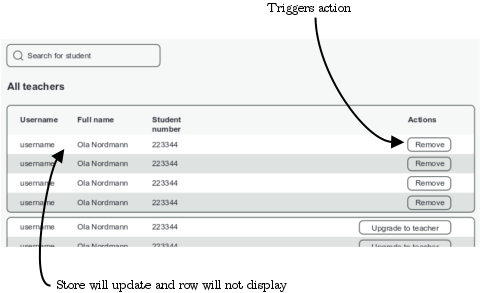
\includegraphics[width=1\linewidth]{graphics/simpleremoveuser.png}}}
  \caption{Wireframe representation of course student list view}
  \label{fig:simpleremoveuser}
\end{figure}

At any given time the application is in some \emph{state}, the state has the information about who is pressing the button, what course is active and much more. When an action to remove a student is being sent, it gets dispatched through a dispatcher (the origin of all changes). The stores that are interested in this action update themselves according to the information in action's payload, slightly changing the state of the application. In this case, one of \emph{action creators} methods, will be sending an action for removing the user from a course.

\begin{figure}[h]
  \scalebox{0.8}{% Graphic for TeX using PGF
% Title: /home/tomgli/workspace/github.com/bachopp/thesis/files/chapters/design/graphics/simplefluxremoveuser.dia
% Creator: Dia v0.97.3
% CreationDate: Mon May  9 16:46:25 2016
% For: tomgli
% \usepackage{tikz}
% The following commands are not supported in PSTricks at present
% We define them conditionally, so when they are implemented,
% this pgf file will use them.
\ifx\du\undefined
  \newlength{\du}
\fi
\setlength{\du}{15\unitlength}
\begin{tikzpicture}
\pgftransformxscale{1.000000}
\pgftransformyscale{-1.000000}
\definecolor{dialinecolor}{rgb}{0.000000, 0.000000, 0.000000}
\pgfsetstrokecolor{dialinecolor}
\definecolor{dialinecolor}{rgb}{1.000000, 1.000000, 1.000000}
\pgfsetfillcolor{dialinecolor}
\definecolor{dialinecolor}{rgb}{1.000000, 1.000000, 1.000000}
\pgfsetfillcolor{dialinecolor}
\fill (28.244400\du,5.226760\du)--(28.244400\du,8.828152\du)--(35.463246\du,8.828152\du)--(35.463246\du,5.226760\du)--cycle;
\pgfsetlinewidth{0.100000\du}
\pgfsetdash{}{0pt}
\pgfsetdash{}{0pt}
\pgfsetmiterjoin
\definecolor{dialinecolor}{rgb}{0.000000, 0.000000, 0.000000}
\pgfsetstrokecolor{dialinecolor}
\draw (28.244400\du,5.226760\du)--(28.244400\du,8.828152\du)--(35.463246\du,8.828152\du)--(35.463246\du,5.226760\du)--cycle;
% setfont left to latex
\definecolor{dialinecolor}{rgb}{0.000000, 0.000000, 0.000000}
\pgfsetstrokecolor{dialinecolor}
\node at (31.853823\du,6.827456\du){View};
% setfont left to latex
\definecolor{dialinecolor}{rgb}{0.000000, 0.000000, 0.000000}
\pgfsetstrokecolor{dialinecolor}
\node at (31.853823\du,7.627456\du){CourseStudentList};
\definecolor{dialinecolor}{rgb}{1.000000, 1.000000, 1.000000}
\pgfsetfillcolor{dialinecolor}
\fill (3.713580\du,5.237260\du)--(3.713580\du,8.838652\du)--(10.103987\du,8.838652\du)--(10.103987\du,5.237260\du)--cycle;
\pgfsetlinewidth{0.100000\du}
\pgfsetdash{}{0pt}
\pgfsetdash{}{0pt}
\pgfsetmiterjoin
\definecolor{dialinecolor}{rgb}{0.000000, 0.000000, 0.000000}
\pgfsetstrokecolor{dialinecolor}
\draw (3.713580\du,5.237260\du)--(3.713580\du,8.838652\du)--(10.103987\du,8.838652\du)--(10.103987\du,5.237260\du)--cycle;
% setfont left to latex
\definecolor{dialinecolor}{rgb}{0.000000, 0.000000, 0.000000}
\pgfsetstrokecolor{dialinecolor}
\node at (6.908784\du,6.837956\du){ActionCreators};
% setfont left to latex
\definecolor{dialinecolor}{rgb}{0.000000, 0.000000, 0.000000}
\pgfsetstrokecolor{dialinecolor}
\node at (6.908784\du,7.637956\du){CourseUsers};
\definecolor{dialinecolor}{rgb}{0.898039, 0.898039, 0.898039}
\pgfsetfillcolor{dialinecolor}
\fill (11.306400\du,5.231230\du)--(11.306400\du,8.832622\du)--(15.403900\du,8.832622\du)--(15.403900\du,5.231230\du)--cycle;
\pgfsetlinewidth{0.100000\du}
\pgfsetdash{}{0pt}
\pgfsetdash{}{0pt}
\pgfsetmiterjoin
\definecolor{dialinecolor}{rgb}{0.000000, 0.000000, 0.000000}
\pgfsetstrokecolor{dialinecolor}
\draw (11.306400\du,5.231230\du)--(11.306400\du,8.832622\du)--(15.403900\du,8.832622\du)--(15.403900\du,5.231230\du)--cycle;
% setfont left to latex
\definecolor{dialinecolor}{rgb}{0.000000, 0.000000, 0.000000}
\pgfsetstrokecolor{dialinecolor}
\node at (13.355150\du,7.231926\du){Dispatcher};
\definecolor{dialinecolor}{rgb}{1.000000, 1.000000, 1.000000}
\pgfsetfillcolor{dialinecolor}
\fill (18.614900\du,5.221790\du)--(18.614900\du,8.823182\du)--(25.313365\du,8.823182\du)--(25.313365\du,5.221790\du)--cycle;
\pgfsetlinewidth{0.100000\du}
\pgfsetdash{}{0pt}
\pgfsetdash{}{0pt}
\pgfsetmiterjoin
\definecolor{dialinecolor}{rgb}{0.000000, 0.000000, 0.000000}
\pgfsetstrokecolor{dialinecolor}
\draw (18.614900\du,5.221790\du)--(18.614900\du,8.823182\du)--(25.313365\du,8.823182\du)--(25.313365\du,5.221790\du)--cycle;
% setfont left to latex
\definecolor{dialinecolor}{rgb}{0.000000, 0.000000, 0.000000}
\pgfsetstrokecolor{dialinecolor}
\node at (21.964132\du,6.822486\du){CourseStudent};
% setfont left to latex
\definecolor{dialinecolor}{rgb}{0.000000, 0.000000, 0.000000}
\pgfsetstrokecolor{dialinecolor}
\node at (21.964132\du,7.622486\du){ListStore};
\pgfsetlinewidth{0.100000\du}
\pgfsetdash{}{0pt}
\pgfsetdash{}{0pt}
\pgfsetbuttcap
{
\definecolor{dialinecolor}{rgb}{0.000000, 0.000000, 0.000000}
\pgfsetfillcolor{dialinecolor}
% was here!!!
\pgfsetarrowsend{latex}
\definecolor{dialinecolor}{rgb}{0.000000, 0.000000, 0.000000}
\pgfsetstrokecolor{dialinecolor}
\draw (10.104000\du,7.037960\du)--(11.306400\du,7.031930\du);
}
\pgfsetlinewidth{0.100000\du}
\pgfsetdash{}{0pt}
\pgfsetdash{}{0pt}
\pgfsetbuttcap
{
\definecolor{dialinecolor}{rgb}{0.000000, 0.000000, 0.000000}
\pgfsetfillcolor{dialinecolor}
% was here!!!
\pgfsetarrowsend{latex}
\definecolor{dialinecolor}{rgb}{0.000000, 0.000000, 0.000000}
\pgfsetstrokecolor{dialinecolor}
\draw (15.403900\du,7.031930\du)--(18.614900\du,7.022486\du);
}
\pgfsetlinewidth{0.100000\du}
\pgfsetdash{}{0pt}
\pgfsetdash{}{0pt}
\pgfsetmiterjoin
\pgfsetbuttcap
{
\definecolor{dialinecolor}{rgb}{0.000000, 0.000000, 0.000000}
\pgfsetfillcolor{dialinecolor}
% was here!!!
\pgfsetarrowsend{latex}
{\pgfsetcornersarced{\pgfpoint{0.000000\du}{0.000000\du}}\definecolor{dialinecolor}{rgb}{0.000000, 0.000000, 0.000000}
\pgfsetstrokecolor{dialinecolor}
\draw (31.853823\du,5.226760\du)--(31.853823\du,4.176760\du)--(6.908784\du,4.176760\du)--(6.908784\du,5.237260\du);
}}
% setfont left to latex
\definecolor{dialinecolor}{rgb}{0.000000, 0.000000, 0.000000}
\pgfsetstrokecolor{dialinecolor}
\node at (19.890111\du,2.751733\du){removeUser()};
% setfont left to latex
\definecolor{dialinecolor}{rgb}{0.000000, 0.000000, 0.000000}
\pgfsetstrokecolor{dialinecolor}
\node at (19.890111\du,3.551733\du){actionType: REMOVE\_USER\_FROM\_COURSE, payload: \{...\}};
% setfont left to latex
\definecolor{dialinecolor}{rgb}{0.000000, 0.000000, 0.000000}
\pgfsetstrokecolor{dialinecolor}
\node at (26.513300\du,6.488150\du){Update};
\pgfsetlinewidth{0.100000\du}
\pgfsetdash{}{0pt}
\pgfsetdash{}{0pt}
\pgfsetbuttcap
{
\definecolor{dialinecolor}{rgb}{0.000000, 0.000000, 0.000000}
\pgfsetfillcolor{dialinecolor}
% was here!!!
\pgfsetarrowsend{latex}
\definecolor{dialinecolor}{rgb}{0.000000, 0.000000, 0.000000}
\pgfsetstrokecolor{dialinecolor}
\draw (25.313365\du,7.022486\du)--(28.244400\du,7.027450\du);
}
% setfont left to latex
\definecolor{dialinecolor}{rgb}{0.000000, 0.000000, 0.000000}
\pgfsetstrokecolor{dialinecolor}
\node at (16.996300\du,6.500290\du){Dispatch};
\definecolor{dialinecolor}{rgb}{1.000000, 1.000000, 1.000000}
\pgfsetfillcolor{dialinecolor}
\pgfpathellipse{\pgfpoint{21.958513\du}{10.950722\du}}{\pgfpoint{3.122513\du}{0\du}}{\pgfpoint{0\du}{1.210632\du}}
\pgfusepath{fill}
\pgfsetlinewidth{0.100000\du}
\pgfsetdash{}{0pt}
\pgfsetdash{}{0pt}
\pgfsetmiterjoin
\definecolor{dialinecolor}{rgb}{0.000000, 0.000000, 0.000000}
\pgfsetstrokecolor{dialinecolor}
\pgfpathellipse{\pgfpoint{21.958513\du}{10.950722\du}}{\pgfpoint{3.122513\du}{0\du}}{\pgfpoint{0\du}{1.210632\du}}
\pgfusepath{stroke}
% setfont left to latex
\definecolor{dialinecolor}{rgb}{0.000000, 0.000000, 0.000000}
\pgfsetstrokecolor{dialinecolor}
\node at (21.958513\du,11.150722\du){update itself};
\pgfsetlinewidth{0.100000\du}
\pgfsetdash{}{0pt}
\pgfsetdash{}{0pt}
\pgfsetbuttcap
{
\definecolor{dialinecolor}{rgb}{0.000000, 0.000000, 0.000000}
\pgfsetfillcolor{dialinecolor}
% was here!!!
\definecolor{dialinecolor}{rgb}{0.000000, 0.000000, 0.000000}
\pgfsetstrokecolor{dialinecolor}
\draw (21.964132\du,8.823182\du)--(21.958500\du,9.740090\du);
}
\end{tikzpicture}
}
  \caption{How removing user happens with this architecture.}
  \label{fig:simplefluxremoveuser}
\end{figure}

Pressing the button to remove a user, will call \emph{removeUser()} from ActionCreatorsCourseUsers, this method will return a object literal, with an \emph{actionType} and \emph{payload} (see Figure \ref{fig:simplefluxremoveuser}), and also pass it further to the Dispatcher. The payload is a coma separated list of variables, in this case only the user data would have to be sent. When the action reaches the store, the store then updates itself, by calling it's private method to manipulate the data it stores. Here is where the \emph{EventEmitter} comes to play, when the stores private methods return, the event emitter assigned to that store emits a \emph{change event}. React components are set up to trigger new render cycles when they receive that change event. What changed doesn't matter, components only needs to know that something changed. When new render cycle is triggered the view will use store's public methods to retrieve new data. This time around the store updated itself to remove the user, as a result the view won't render that user in this render cycle.

\subsection{Advanced Flux}\label{sec:advancedfluxexample}
What makes Flux a great architecture is that more complicated implementations do not differ that much form the simpler ones. The data flow in Flux is one directional, two different views won't communicate directly with eachother, rather they will do so by creating actions, triggering store changes and consequently updating both views. To explain how different views communicate, and how stores and store dependencies work, it is necessary to look at a bigger part of a page not just one single element, and explore the communication between views making up that page.
\\Lets take a look at the views responsible for managing groups for courses. There are three main views shown in figure \ref{fig:advancedgroupmanager}, first takes care of switching between the courses, second lists available students that have no groups assigned, and the last one shows group list and manager. The first view at the top, is for switching between courses, it's independent of the two views below it. Switching course will change the state of the application consequently triggering an API request for new list of students and groups. The buttons for adding students to course, on the left view, and data associated with them, communicate with the right view that lists the groups and participants.

\todo{numerate figure elements}
\begin{figure}[h]
 % \scalebox{1}{% Graphic for TeX using PGF
% Title: /home/tomgli/workspace/github.com/bachopp/thesis/files/chapters/design/graphics/simpleremoveuser.dia
% Creator: Dia v0.97.3
% CreationDate: Fri May  6 18:21:29 2016
% For: tomgli
% \usepackage{tikz}
% The following commands are not supported in PSTricks at present
% We define them conditionally, so when they are implemented,
% this pgf file will use them.
\ifx\du\undefined
  \newlength{\du}
\fi
\setlength{\du}{15\unitlength}
\begin{tikzpicture}
\pgftransformxscale{1.000000}
\pgftransformyscale{-1.000000}
\definecolor{dialinecolor}{rgb}{0.000000, 0.000000, 0.000000}
\pgfsetstrokecolor{dialinecolor}
\definecolor{dialinecolor}{rgb}{1.000000, 1.000000, 1.000000}
\pgfsetfillcolor{dialinecolor}
% image rendering not supported% setfont left to latex
\definecolor{dialinecolor}{rgb}{0.000000, 0.000000, 0.000000}
\pgfsetstrokecolor{dialinecolor}
\node at (48.662500\du,24.782500\du){Triggers action};
\pgfsetlinewidth{0.100000\du}
\pgfsetdash{}{0pt}
\pgfsetdash{}{0pt}
\pgfsetmiterjoin
\pgfsetbuttcap
{
\definecolor{dialinecolor}{rgb}{0.000000, 0.000000, 0.000000}
\pgfsetfillcolor{dialinecolor}
% was here!!!
\pgfsetarrowsend{latex}
\definecolor{dialinecolor}{rgb}{0.000000, 0.000000, 0.000000}
\pgfsetstrokecolor{dialinecolor}
\pgfpathmoveto{\pgfpoint{48.887500\du}{25.062500\du}}
\pgfpathcurveto{\pgfpoint{48.937500\du}{27.862500\du}}{\pgfpoint{51.420701\du}{31.239594\du}}{\pgfpoint{53.268638\du}{31.296658\du}}
\pgfusepath{stroke}
}
% setfont left to latex
\definecolor{dialinecolor}{rgb}{0.000000, 0.000000, 0.000000}
\pgfsetstrokecolor{dialinecolor}
\node[anchor=west] at (35.901642\du,38.651596\du){Store will update and row will not display};
\pgfsetlinewidth{0.100000\du}
\pgfsetdash{}{0pt}
\pgfsetdash{}{0pt}
\pgfsetmiterjoin
\pgfsetbuttcap
{
\definecolor{dialinecolor}{rgb}{0.000000, 0.000000, 0.000000}
\pgfsetfillcolor{dialinecolor}
% was here!!!
\pgfsetarrowsend{latex}
\definecolor{dialinecolor}{rgb}{0.000000, 0.000000, 0.000000}
\pgfsetstrokecolor{dialinecolor}
\pgfpathmoveto{\pgfpoint{35.638700\du}{38.461607\du}}
\pgfpathcurveto{\pgfpoint{34.483865\du}{38.461607\du}}{\pgfpoint{35.490050\du}{32.812892\du}}{\pgfpoint{36.292762\du}{31.683149\du}}
\pgfusepath{stroke}
}
\end{tikzpicture}
}
  \scalebox{1}[1]{{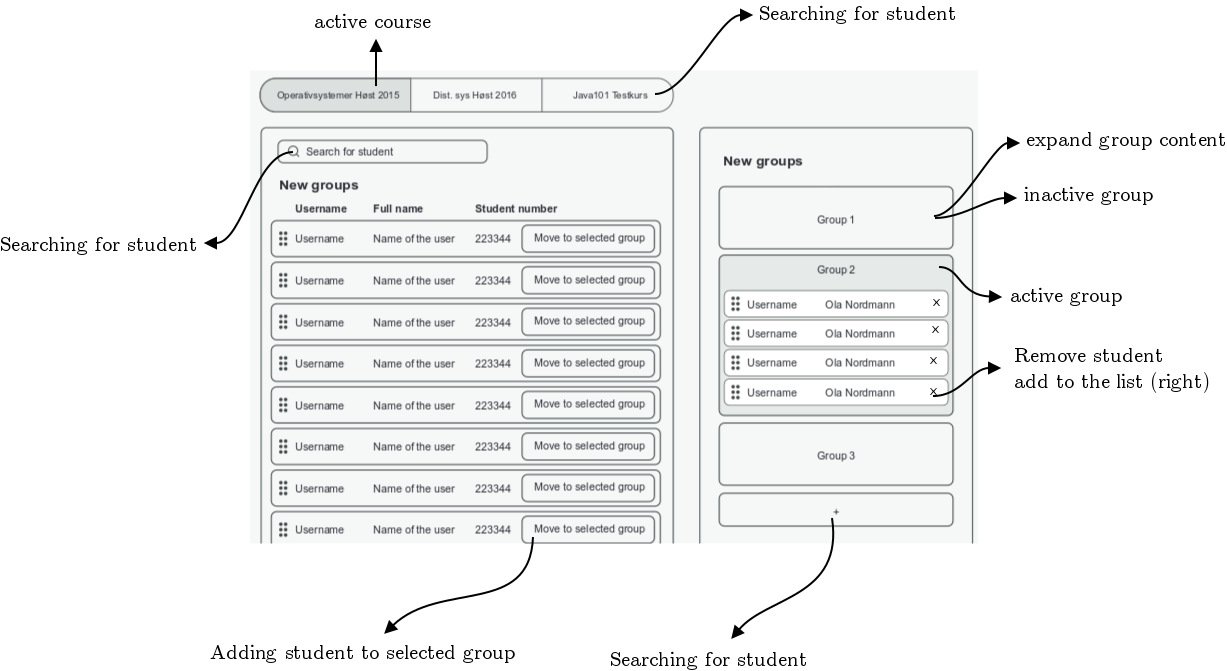
\includegraphics[width=1\linewidth]{graphics/advancedgroupmanager.png}}}
  \caption{Group manager and actions that can be triggered by user}
  \todo{fix figure}
  \label{fig:advancedgroupmanager}
\end{figure}

Datastructure that will represent the two views, a store called \emph{GroupManagerStore}, will have to communicate with another store \emph{ActiveCourseStore} - that store is responsible for holding data about the current active course in the state. In this particular example, GroupManagerStore depends on the data in ActiveCourseStore. However we don't have to worry about ActiveCouresStore being empty, what could trigger an \emph{exception}, since there is always a course that is active. In addition to those two stores, a third store is used in the background. Given that a teacher selected a course, he will most likely stay on that course in order to execute different changes in that course. This gives an opportunity to optimize the API requests to some degree. The student data for the current course can be reused  while the user navigates within a course. Therefore there is a separate store for student list called \emph{StudentsStore}, other stores that require a list of students will no longer have to request this data from the server, given that another store already requested student lists and the user didn't switch the course. For example, both GroupManagerStore and the store from previous example \ref{sec:simplefluxexample} would require a list of students, if navigation between views utilizing those views will take place only one initial API request will be triggered.
\\Given the state shown in figure \ref{fig:advancedgroupmanager}, the teacher selects a user to be added to the active course, lets go through the flow of data in that case.

\begin{figure}[h]
  \scalebox{0.8}{% Graphic for TeX using PGF
% Title: /home/tomgli/workspace/github.com/bachopp/thesis/files/chapters/design/graphics/advancedfluxaddstudent.dia
% Creator: Dia v0.97.3
% CreationDate: Tue May 10 18:29:14 2016
% For: tomgli
% \usepackage{tikz}
% The following commands are not supported in PSTricks at present
% We define them conditionally, so when they are implemented,
% this pgf file will use them.
\ifx\du\undefined
  \newlength{\du}
\fi
\setlength{\du}{15\unitlength}
\begin{tikzpicture}
\pgftransformxscale{1.000000}
\pgftransformyscale{-1.000000}
\definecolor{dialinecolor}{rgb}{0.000000, 0.000000, 0.000000}
\pgfsetstrokecolor{dialinecolor}
\definecolor{dialinecolor}{rgb}{1.000000, 1.000000, 1.000000}
\pgfsetfillcolor{dialinecolor}
\definecolor{dialinecolor}{rgb}{1.000000, 1.000000, 1.000000}
\pgfsetfillcolor{dialinecolor}
\fill (3.410616\du,5.205062\du)--(3.410616\du,8.806454\du)--(9.000991\du,8.806454\du)--(9.000991\du,5.205062\du)--cycle;
\pgfsetlinewidth{0.100000\du}
\pgfsetdash{}{0pt}
\pgfsetdash{}{0pt}
\pgfsetmiterjoin
\definecolor{dialinecolor}{rgb}{0.000000, 0.000000, 0.000000}
\pgfsetstrokecolor{dialinecolor}
\draw (3.410616\du,5.205062\du)--(3.410616\du,8.806454\du)--(9.000991\du,8.806454\du)--(9.000991\du,5.205062\du)--cycle;
% setfont left to latex
\definecolor{dialinecolor}{rgb}{0.000000, 0.000000, 0.000000}
\pgfsetstrokecolor{dialinecolor}
\node at (6.205804\du,6.805758\du){GroupManager};
% setfont left to latex
\definecolor{dialinecolor}{rgb}{0.000000, 0.000000, 0.000000}
\pgfsetstrokecolor{dialinecolor}
\node at (6.205804\du,7.605758\du){ActionCreators};
\definecolor{dialinecolor}{rgb}{0.945098, 0.945098, 0.945098}
\pgfsetfillcolor{dialinecolor}
\fill (10.661200\du,5.194684\du)--(10.661200\du,8.796076\du)--(15.166074\du,8.796076\du)--(15.166074\du,5.194684\du)--cycle;
\pgfsetlinewidth{0.100000\du}
\pgfsetdash{}{0pt}
\pgfsetdash{}{0pt}
\pgfsetmiterjoin
\definecolor{dialinecolor}{rgb}{0.000000, 0.000000, 0.000000}
\pgfsetstrokecolor{dialinecolor}
\draw (10.661200\du,5.194684\du)--(10.661200\du,8.796076\du)--(15.166074\du,8.796076\du)--(15.166074\du,5.194684\du)--cycle;
% setfont left to latex
\definecolor{dialinecolor}{rgb}{0.000000, 0.000000, 0.000000}
\pgfsetstrokecolor{dialinecolor}
\node[anchor=east] at (14.716074\du,7.195380\du){Dispatcher};
\pgfsetlinewidth{0.100000\du}
\pgfsetdash{}{0pt}
\pgfsetdash{}{0pt}
\pgfsetbuttcap
{
\definecolor{dialinecolor}{rgb}{0.000000, 0.000000, 0.000000}
\pgfsetfillcolor{dialinecolor}
% was here!!!
\pgfsetarrowsend{latex}
\definecolor{dialinecolor}{rgb}{0.000000, 0.000000, 0.000000}
\pgfsetstrokecolor{dialinecolor}
\draw (9.000991\du,7.005758\du)--(10.661200\du,6.995380\du);
}
\pgfsetlinewidth{0.100000\du}
\pgfsetdash{}{0pt}
\pgfsetdash{}{0pt}
\pgfsetmiterjoin
\pgfsetbuttcap
{
\definecolor{dialinecolor}{rgb}{0.000000, 0.000000, 0.000000}
\pgfsetfillcolor{dialinecolor}
% was here!!!
\pgfsetarrowsend{latex}
{\pgfsetcornersarced{\pgfpoint{0.000000\du}{0.000000\du}}\definecolor{dialinecolor}{rgb}{0.000000, 0.000000, 0.000000}
\pgfsetstrokecolor{dialinecolor}
\draw (32.886300\du,4.175120\du)--(32.886300\du,2.204767\du)--(6.205804\du,2.204767\du)--(6.205804\du,5.205062\du);
}}
% setfont left to latex
\definecolor{dialinecolor}{rgb}{0.000000, 0.000000, 0.000000}
\pgfsetstrokecolor{dialinecolor}
\node[anchor=west] at (8.203756\du,0.130673\du){actionType: ADD\_USER\_TO\_GROUP, payload: \{};
% setfont left to latex
\definecolor{dialinecolor}{rgb}{0.000000, 0.000000, 0.000000}
\pgfsetstrokecolor{dialinecolor}
\node[anchor=west] at (8.203756\du,0.930673\du){                                                                      user:\{ name:"test", ... \},};
% setfont left to latex
\definecolor{dialinecolor}{rgb}{0.000000, 0.000000, 0.000000}
\pgfsetstrokecolor{dialinecolor}
\node[anchor=west] at (8.203756\du,1.730673\du){                                                                     \}};
% setfont left to latex
\definecolor{dialinecolor}{rgb}{0.000000, 0.000000, 0.000000}
\pgfsetstrokecolor{dialinecolor}
\node at (28.881375\du,7.103016\du){Update};
% setfont left to latex
\definecolor{dialinecolor}{rgb}{0.000000, 0.000000, 0.000000}
\pgfsetstrokecolor{dialinecolor}
\node at (17.266200\du,6.615950\du){Dispatch};
\definecolor{dialinecolor}{rgb}{1.000000, 1.000000, 1.000000}
\pgfsetfillcolor{dialinecolor}
\fill (30.348400\du,7.095990\du)--(30.348400\du,9.795990\du)--(35.396282\du,9.795990\du)--(35.396282\du,7.095990\du)--cycle;
\pgfsetlinewidth{0.100000\du}
\pgfsetdash{}{0pt}
\pgfsetdash{}{0pt}
\pgfsetmiterjoin
\definecolor{dialinecolor}{rgb}{0.000000, 0.000000, 0.000000}
\pgfsetstrokecolor{dialinecolor}
\draw (30.348400\du,7.095990\du)--(30.348400\du,9.795990\du)--(35.396282\du,9.795990\du)--(35.396282\du,7.095990\du)--cycle;
% setfont left to latex
\definecolor{dialinecolor}{rgb}{0.000000, 0.000000, 0.000000}
\pgfsetstrokecolor{dialinecolor}
\node at (32.872341\du,8.245990\du){View};
% setfont left to latex
\definecolor{dialinecolor}{rgb}{0.000000, 0.000000, 0.000000}
\pgfsetstrokecolor{dialinecolor}
\node at (32.872341\du,9.045990\du){GroupList};
\pgfsetlinewidth{0.100000\du}
\pgfsetdash{}{0pt}
\pgfsetdash{}{0pt}
\pgfsetmiterjoin
\pgfsetbuttcap
{
\definecolor{dialinecolor}{rgb}{0.000000, 0.000000, 0.000000}
\pgfsetfillcolor{dialinecolor}
% was here!!!
\pgfsetarrowsend{latex}
\definecolor{dialinecolor}{rgb}{0.000000, 0.000000, 0.000000}
\pgfsetstrokecolor{dialinecolor}
\pgfpathmoveto{\pgfpoint{26.567545\du}{6.989366\du}}
\pgfpathcurveto{\pgfpoint{27.781345\du}{6.989366\du}}{\pgfpoint{29.148500\du}{5.525120\du}}{\pgfpoint{30.362300\du}{5.525120\du}}
\pgfusepath{stroke}
}
\pgfsetlinewidth{0.100000\du}
\pgfsetdash{}{0pt}
\pgfsetdash{}{0pt}
\pgfsetmiterjoin
\pgfsetbuttcap
{
\definecolor{dialinecolor}{rgb}{0.000000, 0.000000, 0.000000}
\pgfsetfillcolor{dialinecolor}
% was here!!!
\pgfsetarrowsend{latex}
\definecolor{dialinecolor}{rgb}{0.000000, 0.000000, 0.000000}
\pgfsetstrokecolor{dialinecolor}
\pgfpathmoveto{\pgfpoint{26.567545\du}{6.989366\du}}
\pgfpathcurveto{\pgfpoint{27.797545\du}{6.989366\du}}{\pgfpoint{29.118400\du}{8.445990\du}}{\pgfpoint{30.348400\du}{8.445990\du}}
\pgfusepath{stroke}
}
\definecolor{dialinecolor}{rgb}{0.815686, 0.815686, 0.815686}
\pgfsetfillcolor{dialinecolor}
\fill (19.605800\du,8.416370\du)--(19.605800\du,11.230157\du)--(26.299423\du,11.230157\du)--(26.299423\du,8.416370\du)--cycle;
\pgfsetlinewidth{0.100000\du}
\pgfsetdash{}{0pt}
\pgfsetdash{}{0pt}
\pgfsetmiterjoin
\definecolor{dialinecolor}{rgb}{0.000000, 0.000000, 0.000000}
\pgfsetstrokecolor{dialinecolor}
\draw (19.605800\du,8.416370\du)--(19.605800\du,11.230157\du)--(26.299423\du,11.230157\du)--(26.299423\du,8.416370\du)--cycle;
% setfont left to latex
\definecolor{dialinecolor}{rgb}{0.000000, 0.000000, 0.000000}
\pgfsetstrokecolor{dialinecolor}
\node at (22.952612\du,10.023263\du){StudentsStore};
\definecolor{dialinecolor}{rgb}{0.945098, 0.945098, 0.945098}
\pgfsetfillcolor{dialinecolor}
\fill (19.528700\du,2.834900\du)--(19.528700\du,5.648687\du)--(26.231030\du,5.648687\du)--(26.231030\du,2.834900\du)--cycle;
\pgfsetlinewidth{0.100000\du}
\pgfsetdash{}{0pt}
\pgfsetdash{}{0pt}
\pgfsetmiterjoin
\definecolor{dialinecolor}{rgb}{0.000000, 0.000000, 0.000000}
\pgfsetstrokecolor{dialinecolor}
\draw (19.528700\du,2.834900\du)--(19.528700\du,5.648687\du)--(26.231030\du,5.648687\du)--(26.231030\du,2.834900\du)--cycle;
% setfont left to latex
\definecolor{dialinecolor}{rgb}{0.000000, 0.000000, 0.000000}
\pgfsetstrokecolor{dialinecolor}
\node at (22.879865\du,4.441793\du){ActiveCourseStore};
\definecolor{dialinecolor}{rgb}{0.701961, 0.701961, 0.701961}
\pgfsetfillcolor{dialinecolor}
\fill (19.220200\du,5.188670\du)--(19.220200\du,8.790062\du)--(26.567545\du,8.790062\du)--(26.567545\du,5.188670\du)--cycle;
\pgfsetlinewidth{0.100000\du}
\pgfsetdash{}{0pt}
\pgfsetdash{}{0pt}
\pgfsetmiterjoin
\definecolor{dialinecolor}{rgb}{0.000000, 0.000000, 0.000000}
\pgfsetstrokecolor{dialinecolor}
\draw (19.220200\du,5.188670\du)--(19.220200\du,8.790062\du)--(26.567545\du,8.790062\du)--(26.567545\du,5.188670\du)--cycle;
% setfont left to latex
\definecolor{dialinecolor}{rgb}{0.000000, 0.000000, 0.000000}
\pgfsetstrokecolor{dialinecolor}
\node at (22.893873\du,7.189366\du){GroupManagerStore};
\definecolor{dialinecolor}{rgb}{1.000000, 1.000000, 1.000000}
\pgfsetfillcolor{dialinecolor}
\fill (30.362300\du,4.175120\du)--(30.362300\du,6.875120\du)--(35.410182\du,6.875120\du)--(35.410182\du,4.175120\du)--cycle;
\pgfsetlinewidth{0.100000\du}
\pgfsetdash{}{0pt}
\pgfsetdash{}{0pt}
\pgfsetmiterjoin
\definecolor{dialinecolor}{rgb}{0.000000, 0.000000, 0.000000}
\pgfsetstrokecolor{dialinecolor}
\draw (30.362300\du,4.175120\du)--(30.362300\du,6.875120\du)--(35.410182\du,6.875120\du)--(35.410182\du,4.175120\du)--cycle;
% setfont left to latex
\definecolor{dialinecolor}{rgb}{0.000000, 0.000000, 0.000000}
\pgfsetstrokecolor{dialinecolor}
\node at (32.886241\du,5.325120\du){View};
% setfont left to latex
\definecolor{dialinecolor}{rgb}{0.000000, 0.000000, 0.000000}
\pgfsetstrokecolor{dialinecolor}
\node at (32.886241\du,6.125120\du){StudentsList};
% setfont left to latex
\definecolor{dialinecolor}{rgb}{0.000000, 0.000000, 0.000000}
\pgfsetstrokecolor{dialinecolor}
\node[anchor=west] at (15.959804\du,13.559443\du){};
% setfont left to latex
\definecolor{dialinecolor}{rgb}{0.000000, 0.000000, 0.000000}
\pgfsetstrokecolor{dialinecolor}
\node[anchor=west] at (13.227467\du,13.483020\du){students = \ensuremath{[}};
% setfont left to latex
\definecolor{dialinecolor}{rgb}{0.000000, 0.000000, 0.000000}
\pgfsetstrokecolor{dialinecolor}
\node[anchor=west] at (13.227467\du,14.283020\du){\{name:"test",...\}};
% setfont left to latex
\definecolor{dialinecolor}{rgb}{0.000000, 0.000000, 0.000000}
\pgfsetstrokecolor{dialinecolor}
\node[anchor=west] at (13.227467\du,15.083020\du){\{name:"test2,...\}};
% setfont left to latex
\definecolor{dialinecolor}{rgb}{0.000000, 0.000000, 0.000000}
\pgfsetstrokecolor{dialinecolor}
\node[anchor=west] at (13.227467\du,15.883020\du){\{...\}};
% setfont left to latex
\definecolor{dialinecolor}{rgb}{0.000000, 0.000000, 0.000000}
\pgfsetstrokecolor{dialinecolor}
\node[anchor=west] at (13.227467\du,16.683020\du){\ensuremath{]}};
\pgfsetlinewidth{0.100000\du}
\pgfsetdash{}{0pt}
\pgfsetdash{}{0pt}
\pgfsetmiterjoin
\pgfsetbuttcap
{
\definecolor{dialinecolor}{rgb}{0.000000, 0.000000, 0.000000}
\pgfsetfillcolor{dialinecolor}
% was here!!!
\pgfsetarrowsend{latex}
\definecolor{dialinecolor}{rgb}{0.000000, 0.000000, 0.000000}
\pgfsetstrokecolor{dialinecolor}
\pgfpathmoveto{\pgfpoint{19.165519\du}{7.913952\du}}
\pgfpathcurveto{\pgfpoint{16.743793\du}{7.900963\du}}{\pgfpoint{16.197224\du}{9.199064\du}}{\pgfpoint{16.213049\du}{12.771493\du}}
\pgfusepath{stroke}
}
% setfont left to latex
\definecolor{dialinecolor}{rgb}{0.000000, 0.000000, 0.000000}
\pgfsetstrokecolor{dialinecolor}
\node at (14.768438\du,11.523947\du){before};
\pgfsetlinewidth{0.100000\du}
\pgfsetdash{}{0pt}
\pgfsetdash{}{0pt}
\pgfsetbuttcap
{
\definecolor{dialinecolor}{rgb}{0.000000, 0.000000, 0.000000}
\pgfsetfillcolor{dialinecolor}
% was here!!!
\pgfsetarrowsend{latex}
\definecolor{dialinecolor}{rgb}{0.000000, 0.000000, 0.000000}
\pgfsetstrokecolor{dialinecolor}
\draw (19.493473\du,14.990278\du)--(22.539314\du,14.990278\du);
}
% setfont left to latex
\definecolor{dialinecolor}{rgb}{0.000000, 0.000000, 0.000000}
\pgfsetstrokecolor{dialinecolor}
\node at (20.654060\du,14.674666\du){update};
% setfont left to latex
\definecolor{dialinecolor}{rgb}{0.000000, 0.000000, 0.000000}
\pgfsetstrokecolor{dialinecolor}
\node[anchor=west] at (23.334563\du,13.481594\du){students = \ensuremath{[}};
% setfont left to latex
\definecolor{dialinecolor}{rgb}{0.000000, 0.000000, 0.000000}
\pgfsetstrokecolor{dialinecolor}
\node[anchor=west] at (23.334563\du,14.281594\du){\{name:"test",...\}};
% setfont left to latex
\definecolor{dialinecolor}{rgb}{0.000000, 0.000000, 0.000000}
\pgfsetstrokecolor{dialinecolor}
\node[anchor=west] at (23.334563\du,15.081594\du){\{name:"test2,...\}};
% setfont left to latex
\definecolor{dialinecolor}{rgb}{0.000000, 0.000000, 0.000000}
\pgfsetstrokecolor{dialinecolor}
\node[anchor=west] at (23.334563\du,15.881594\du){\{...\}};
% setfont left to latex
\definecolor{dialinecolor}{rgb}{0.000000, 0.000000, 0.000000}
\pgfsetstrokecolor{dialinecolor}
\node[anchor=west] at (23.334563\du,16.681594\du){\ensuremath{]}};
\pgfsetlinewidth{0.100000\du}
\pgfsetdash{}{0pt}
\pgfsetdash{}{0pt}
\pgfsetbuttcap
{
\definecolor{dialinecolor}{rgb}{0.000000, 0.000000, 0.000000}
\pgfsetfillcolor{dialinecolor}
% was here!!!
\definecolor{dialinecolor}{rgb}{0.000000, 0.000000, 0.000000}
\pgfsetstrokecolor{dialinecolor}
\draw (23.652346\du,14.293351\du)--(29.397033\du,14.293351\du);
}
\pgfsetlinewidth{0.100000\du}
\pgfsetdash{}{0pt}
\pgfsetdash{}{0pt}
\pgfsetbuttcap
{
\definecolor{dialinecolor}{rgb}{0.000000, 0.000000, 0.000000}
\pgfsetfillcolor{dialinecolor}
% was here!!!
\pgfsetarrowsend{latex}
\definecolor{dialinecolor}{rgb}{0.000000, 0.000000, 0.000000}
\pgfsetstrokecolor{dialinecolor}
\draw (15.166074\du,6.995380\du)--(19.220200\du,6.989366\du);
}
\pgfsetlinewidth{0.100000\du}
\pgfsetdash{{\pgflinewidth}{0.200000\du}}{0cm}
\pgfsetdash{{\pgflinewidth}{0.200000\du}}{0cm}
\pgfsetmiterjoin
\definecolor{dialinecolor}{rgb}{0.000000, 0.000000, 0.000000}
\pgfsetstrokecolor{dialinecolor}
\pgfpathellipse{\pgfpoint{28.664294\du}{7.015184\du}}{\pgfpoint{2.479850\du}{0\du}}{\pgfpoint{0\du}{2.330956\du}}
\pgfusepath{stroke}
% setfont left to latex
\definecolor{dialinecolor}{rgb}{0.000000, 0.000000, 0.000000}
\pgfsetstrokecolor{dialinecolor}
\node at (28.664294\du,7.210184\du){};
\pgfsetlinewidth{0.100000\du}
\pgfsetdash{}{0pt}
\pgfsetdash{}{0pt}
\pgfsetmiterjoin
\pgfsetbuttcap
{
\definecolor{dialinecolor}{rgb}{0.000000, 0.000000, 0.000000}
\pgfsetfillcolor{dialinecolor}
% was here!!!
\pgfsetarrowsstart{latex}
\definecolor{dialinecolor}{rgb}{0.000000, 0.000000, 0.000000}
\pgfsetstrokecolor{dialinecolor}
\pgfpathmoveto{\pgfpoint{28.735545\du}{9.416979\du}}
\pgfpathcurveto{\pgfpoint{28.735220\du}{11.175743\du}}{\pgfpoint{29.380741\du}{11.769586\du}}{\pgfpoint{30.077157\du}{11.769586\du}}
\pgfusepath{stroke}
}
% setfont left to latex
\definecolor{dialinecolor}{rgb}{0.000000, 0.000000, 0.000000}
\pgfsetstrokecolor{dialinecolor}
\node[anchor=west] at (30.253933\du,11.999395\du){EventEmitter};
\end{tikzpicture}
}
  \caption{How removing user happens with this architecture.}
  \label{fig:advancedfluxaddstudent}
\end{figure}

When the user presses the button, one of \emph{GroupManagerActionCreators} is called. The current state, based on the figure \ref{fig:advancedgroupmanager} includes data like:
\\\emph{activeGroup:"Group2",activeCourse:"DAT310" \todo{fix figure and data}}
\\activeGroup field is located in GroupManagerStore, this data represents which group did the user activate, in order to add new student to it. Selected button will have the students data in it's payload, sending it through the Dispatcher, the stores will wait for an actionType to be received. At this point GroupManagerStore sees the actionType, and updates it's students field, the student in the payload gets matched with the existing one in the store and gets removed. Next an update is emitter with the help of EventEmitter, this triggers a new render cycle in the Recat components which consequently get the new data from the stores.
